\documentclass{article}

\usepackage[english]{babel}
\usepackage[utf8]{inputenc}
\usepackage{amsmath}
\usepackage{mathtools}
\usepackage{graphicx}
\usepackage{float}
\usepackage[breaklinks]{hyperref}
\usepackage[font=footnotesize,labelfont=bf,margin=2.5cm,hypcap=false]{caption}
\usepackage{listings}
\usepackage[round]{natbib}
\bibliographystyle{plainnat}


\title{
	Project 03 \\
	\bigskip
	\normalsize APSC 607 Fall 2017
}

\author{Seth Goodman}

\date{\today}


\begin{document}
\maketitle


%\begin{abstract}
%\end{abstract}

\section{Introduction}
\label{sec:introduction}

This project explores different numerical methods of solving two well-posed initial value problems (IVPs), $y'$, at discrete points within a range $[a\ b]$ for a given initial value $y(a)$ as defined in Equation \ref{eq:intro} and described in \cite{burden2010}. The methods that will be tested are Euler's method (i.e., first order Taylor method), fourth order Runge-Kutta (i.e., essentially fourth order Taylor method), and an implicit trapezoidal method (trapezoidal with Newton Iteration). The behavior and characteristics of these methods will be reviewed and their effectiveness evaluated based on the true solution to the IVP.

\begin{equation}
y' = \frac{dy}{dt} = f(t,y), \qquad a \leq t \leq b, \qquad  y(a) = \alpha
\label{eq:intro}
\end{equation}

All computations are performed using MATLAB using the code accompanying this report. Section \ref{sec:methods} will present the methods used in MATLAB to explore functions. Section \ref{sec:results} contains the results and related outputs for each function, and Section \ref{sec:conc} includes discussion and conclusion. All figures and tables found in this report are available in the output subdirectory of the accompanying zip file. Additionally, all code and figures found in the zip file can be accessed via GitHub\footnote{\url{https://github.com/sgoodm/apsc607/tree/master/project_03}}

\newpage
\section{Methods}
\label{sec:methods}

The two unique functions which will be explored in this project, Functions \textbf{A} and \textbf{B}, are defined by Equations \ref{eq:fa} and \ref{eq:fb}, respectively.

\begin{center}
    \centering
    \begin{minipage}{0.5\textwidth}
        \centering
        \begin{equation}
		y' = -9y
		\label{eq:fa}
		\end{equation}
    \end{minipage}\hfill
    \begin{minipage}{0.5\textwidth}
        \centering
        \begin{equation}
        y' = 20 (y-t^2)+2t
		\label{eq:fb}
		\end{equation}
    \end{minipage}
\end{center}


The associated initial values for Functions A and B, are defined by Equations \ref{eq:iva} and \ref{eq:ivb}.


\begin{center}
    \centering
    \begin{minipage}{0.5\textwidth}
        \centering
        \begin{equation}
		y(0) = e
		\label{eq:iva}
		\end{equation}
    \end{minipage}\hfill
    \begin{minipage}{0.5\textwidth}
        \centering
        \begin{equation}
        y(0) = \frac{1}{3}
		\label{eq:ivb}
		\end{equation}
    \end{minipage}
\end{center}


Both IVPs will be examined over the range $ 0 \leq t \leq 1 $, using a baseline step size of $h=0.1$.

To validate and compare each method for solving the IVPs, the true solution is required. The true solution is generated using the Symbolic Toolkit in MATLAB as seen in the example below for Function A.

\bigskip
\begin{lstlisting}[language=Matlab]
	syms y(t)
	ode = diff(y,t) == -9*y;
	cond = y(0) == exp(1);
	sol = dsolve(ode, cond);
\end{lstlisting}
\bigskip

Which produces the functions $y(t)$ for A and B seen in \ref{eq:trueya} and \ref{eq:trueyb}.

\begin{center}
    \centering
    \begin{minipage}{0.5\textwidth}
        \centering
        \begin{equation}
		y(t) = e^{1-9t}
		\label{eq:trueya}
		\end{equation}
    \end{minipage}\hfill
    \begin{minipage}{0.5\textwidth}
        \centering
        \begin{equation}
        y(t) = \frac{1}{3}e^{-20t}+t^2
		\label{eq:trueyb}
		\end{equation}
    \end{minipage}
\end{center}

The true values for Functions A and B are compared to the results from solving the IVP using Euler's method, the fourth order Runge-Kutta method, and the implicit trapezoidal method with Newtonian iteration. In addition to the baseline step size, additional values of \textit{h} will be tested to explore the impact of step size when dealing with stiff equations. 

Stiff IVP equations, as described in \cite{burden2010}, are characterized by having a solution taking the form of $e^{-ct}$. This portion of the solution, known as the \textit{transient solution}, will decay to zero as \textit{t} increases. However, the derivatives of the transient solution take the form $e^{n}e^{-ct}$, which does not decay as quickly as, and can grow very large for small values of \textit{t}. This is inherently problematic when solving IVPs using methods based on Taylor's Theorem or methods with similar error terms, as the derivatives define the error terms. Given that error terms in these methods are evaluated at values between zero and \textit{t}, rather than \textit{t} itself, makes it extremely likely for the derivative of the transient solution to result in large values \citep{burden2010}. Testing IVPs A and B over a range of increasing step sizes, between 0.01 and 0.1, will illustrate the role of step size in the stability of stiff equations when using Euler's or Runge-Kutta methods. Additionally, for each function a considerably larger step size will be tested, at which the error due to the transient solution is substantially larger than the \textit{steady-state} component of the solution. Section \ref{sec:results} will show how implicit methods, such as the implicit trapezoidal with Newtonian iteration that is introduced in this section, can be used as an effective solution to stiff equations without reducing step size.

The remainder of this section will provide details on the implementation of and methods for each of the three approaches to solving IVPs (Euler's, fourth order Runge-Kutta, and the implicit trapezoidal with Newtonian iteration).


\subsection{Euler's (first order Taylor)}
\label{method:euler}
% page 266

\begin{center}
  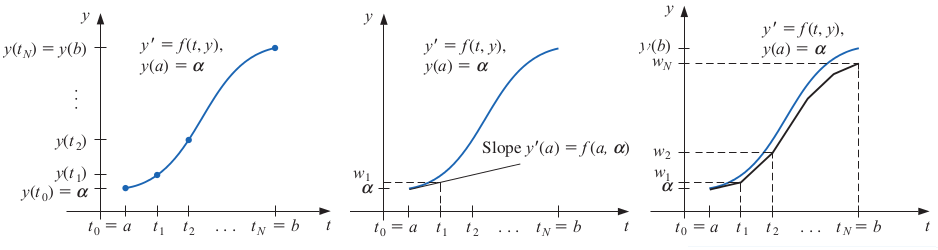
\includegraphics[width=0.9\textwidth]{../additional/euler_method.png}
  \captionof{figure}{Example function (left), single step of Euler's method (center), multiple steps of Euler's method (right). \citep{burden2010}}
  \label{fig:euler_method}
\end{center}

Euler's method is a first order implementation of higher order Taylor's method. Using the initial condition of the function at a given time step \textit{t}, the slope at that point, and the step size, the value of the function at \textit{t+1} can be estimated with second order error (Equation \ref{eq:euler}). This process is illustrated in Figure \ref{fig:euler_method}.

\begin{center}
	\begin{equation}
	y(t_{i+1}) = y(t_i) + hy'(t_i)+\frac{h^2}{2}y''(\xi_i) 
	\label{eq:euler}
	\end{equation}
\end{center}

Given $w_i \approx y(t_i)$ when the error term is removed, Euler's method can be represented by Equation \ref{eq:euleralt}.

\begin{center}
	\begin{equation}
	w_{i+1} = w_i + hf(t_i, w_i)
	\label{eq:euleralt}
	\end{equation}
\end{center}

While Euler's method only requires the first derivative provided with the IVP to solve, using higher order implementations of Taylor's method require additional derivatives. The cost and complexity of having to calculate each subsequent derivative make Taylor's method impractical for use in most applications. The equation for Taylor's method of order \textit{n} can be seen in Equation \ref{eq:taylor}.

\begin{center}
	\begin{equation}
	y(t_{i+1}) = y(t_i) + hy'(t_i)+\frac{h^2}{2}y''(t_i) + \dots + \frac{h^n}{n!}y^{(n)} + \frac{h^{n+1}}{(n+1)!}y^{(n+1)}(\xi_i) 
	\label{eq:taylor}
	\end{equation}
\end{center}


\subsection{Runge-Kutta Order Four}
\label{method:rk}
% page 288

The Runga-Kutta method provides the higher order error term achievable using Taylor's method without the need for additional derivatives in the calculation. This is possible by utilizing the slope of the function at sub steps (e.g., $t_i+0.5h$ within a given step size to better approximate the value of the function at the subsequent time step ($t_{i+1}$).

\begin{center}
	\begin{flalign}
		& k_1 = hf((t_i, w_i), \\
		& k_2 = hf((t_i+\frac{h}{2}, w_i+\frac{1}{2}k_1), \\
		& k_3 = hf((t_i+\frac{h}{2}, w_i+\frac{1}{2}k_2), \\
		& k_4 = hf((t_{i+1}, w_i+k_3), \\
		& w_{i+1} = w_i + \frac{1}{6}(k_1 + 2k_2 + 2k_3 + k_4) 
	\label{eq:rk4}
	\end{flalign}
\end{center}

As seen in the equations below, four \textit{k} values are generated which generate pseudo-approximations of the value at $t_{i+1}$ based on different sub steps and pseudo-starting conditions. The first \textit{k} value is based on the slope and value at $t_i$, the other \textit{k} values use either $t_i+0.5h$ or $t_{i+1}$ along with the value of $w_i$ adjusted by the previously generate \textit{k} values. The final estimate for $w_{i+1}$ combines these to generate a higher order approximation similar to Taylor's method without requiring additional derivatives to be calculated. An illustration of this process depicting the slopes associated with each \textit{k} value, as well as the final slope, can be seen in Figure \ref{fig:rk4_method}.

\begin{center}
  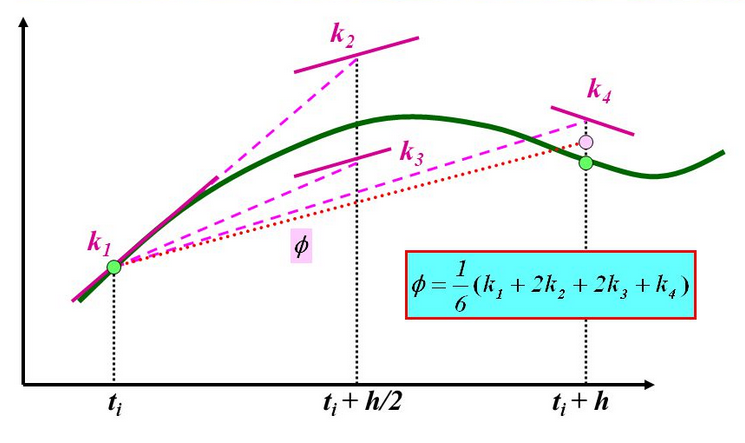
\includegraphics[width=0.7\textwidth]{../additional/rk_method.png}
  \captionof{figure}{Runge-Kutta fourth order illustration. \citep{slide}}
  \label{fig:rk4_method}
\end{center}


\subsection{Implicit Trapezoidal (Trapezoidal with Newtonian Iteration)}
\label{method:implicit}
% page 348

Euler's method, as well as higher order Taylor's method, and Runge-Kutta methods are explicit one-step methods of solving IVPs. As Section \ref{sec:results} will show, these methods suffer from instability when dealing with stiff equations such as Functions A and B used in this project. An alternative is to use an implicit method, such as the implicit trapezoidal with Newtonian iteration (Equation \ref{eq:implcit}, \citep{burden2010}), which utilizes an iterative approach to incorporate information above the current time step ($(t_{i+1}, f(t_{i+1}, w_{i+1}))$) into the approximation. This contrasts to explicit (one-step) methods such as Euler's, Taylor's, and Runga-Kutta, which are based only on a previous time step ($(t_{i}, f(t_{i}, w_{i}))$). 

\begin{center}
	\begin{equation}
	w_{j+1} = w_j + \frac{h}{2} \big[ f(t_{j+1}, w_{j+1}) + f(t_{j}, w_{j}) \big]
	\label{eq:implcit}
	\end{equation}
\end{center}

A simplified pseudo-code implementation of this method can be seen below. For each \textit{t} the \textit{k1} term contains the information about the previous step, while the term within the iterative portion (while loop) is based on current step. The iterative process continues until a specified tolerance has been met (or other conditions are reached - not shown in pseudo code).

\bigskip
\begin{center}
\footnotesize
\begin{lstlisting}[language=Matlab]
    t = a:h:b;
    w(1) = y0;

    for i in t
        k1 = w(i) + 0.5*h * fh(t(i), w(i));
        w0 = k1;
        w0prev = w0;

        while abs(w(i+1)-w0) < TOL
            w0 = w0prev;

            num = w0 - 0.5*h * fh(t(i)+h, w0) - k1;
            den = 1 - 0.5*h * fh'(t(i)+h, w0);
            w(i+1) = w0 - num/den;

            w0prev = w(i+1);
        end    
    end
\end{lstlisting}
\end{center}
\bigskip




\newpage
\section{Results}
\label{sec:results}




This section will review the results for initial value problems and methods presented in Section \ref{sec:methods}. The plots of the functions for the solutions to IVPs A and B can be seen in Figure \ref{fig:true}.

\begin{center}
	\centering
    \begin{minipage}{0.5\textwidth}
        \centering
	    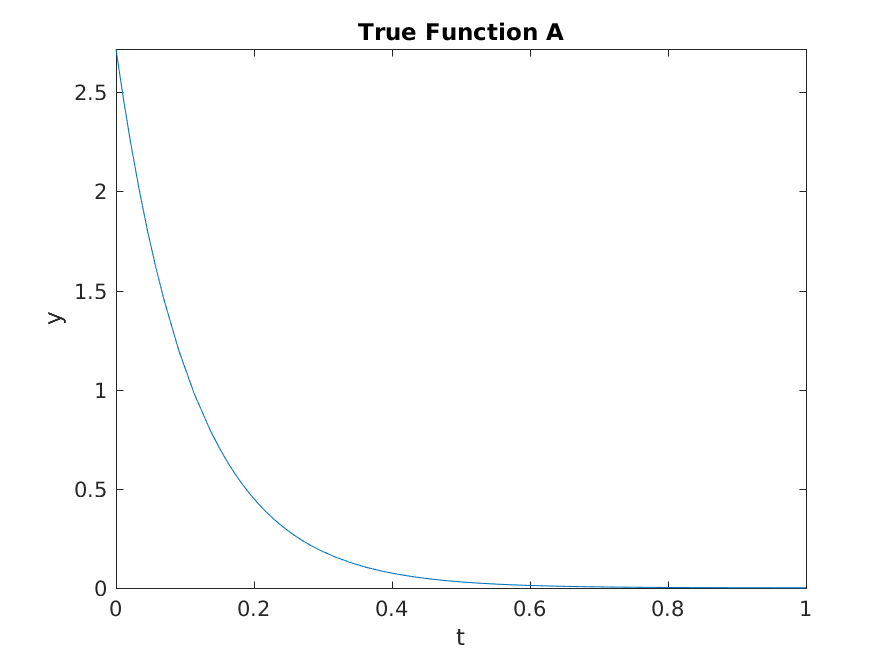
\includegraphics[width=1.1\textwidth]{../output/a_actual.png}
    \end{minipage}\hfill
    \begin{minipage}{0.5\textwidth}
        \centering
	    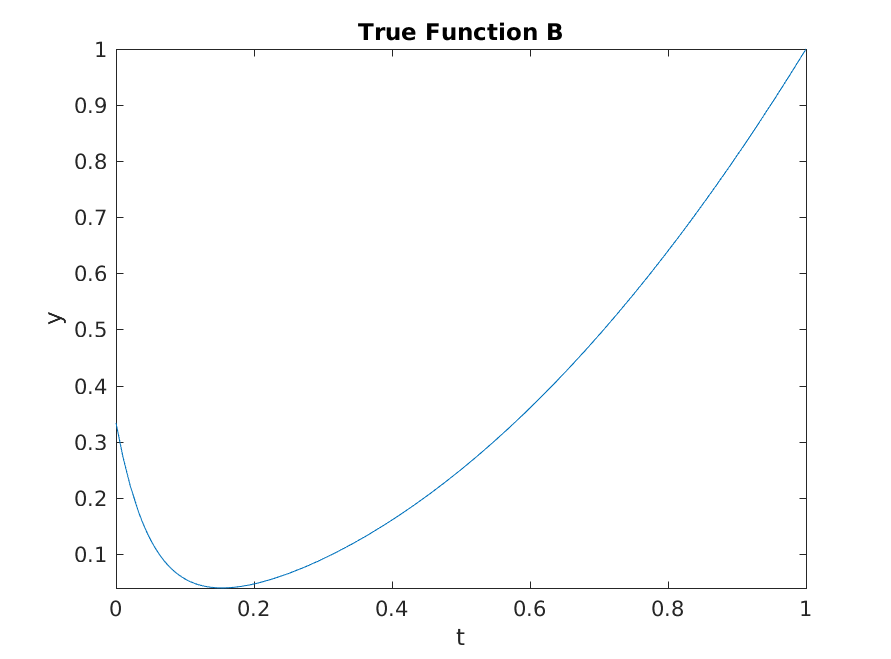
\includegraphics[width=1.1\textwidth]{../output/b_actual.png}
    \end{minipage}
   	\captionof{figure}{True plots of Function A and B between zero and one}
 	\label{fig:true}
\end{center}

The results for each method are plotted simultaneously over a range of step sizes, with the line represent each increasing step size determined based on visible color spectrum, as seen in Figure \ref{fig:h_val_colormap}, with red representing the smallest step size (0.01) and violet the largest (0.1). The increase between step sizes is 0.01. 

\begin{center}
  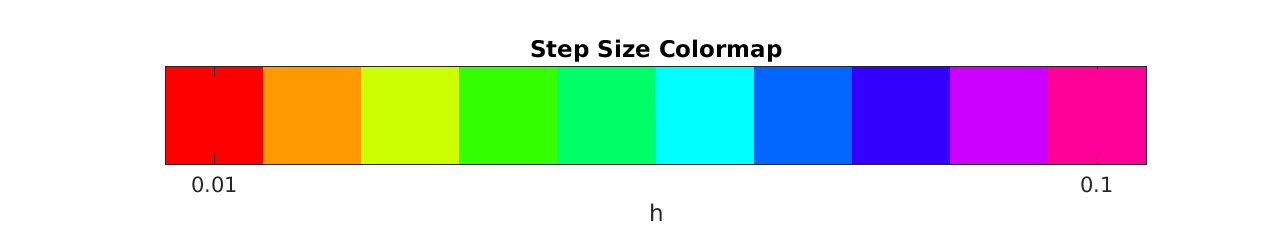
\includegraphics[width=0.9\textwidth]{../output/colormap.png}
  \captionof{figure}{Colormap of h val}
  \label{fig:h_val_colormap}
\end{center}

Results from separate runs which display the behavior of the methods when using significantly larger step sizes (0.2+) with stiff equations will also be shown. The remainder of this section will present these plots and tables of the IVP solution estimates and related error. 


\subsection{Euler's Results}
\label{results:euler}

\begin{center}
	\centering
    \begin{minipage}{0.5\textwidth}
        \centering
	    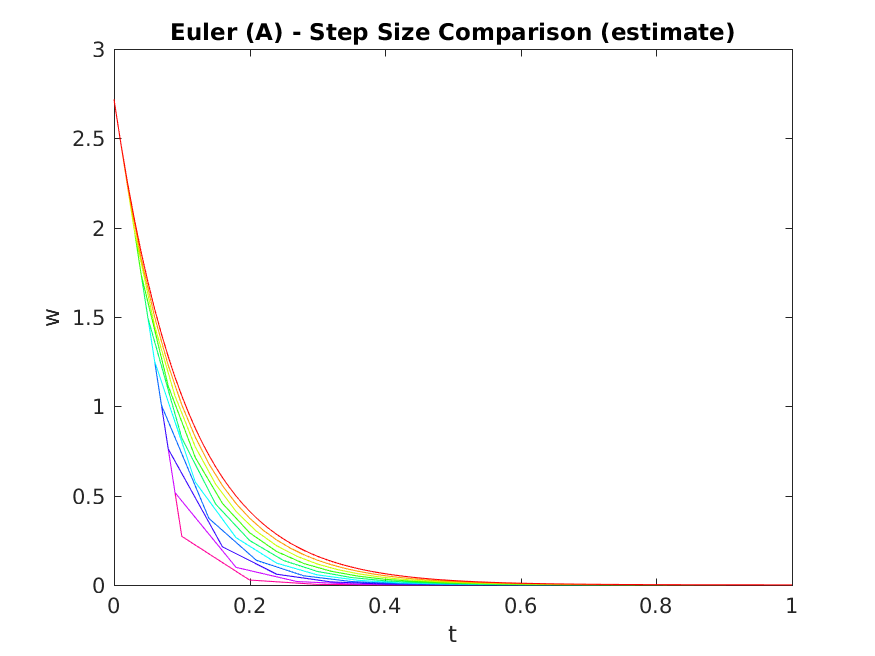
\includegraphics[width=1\textwidth]{../output/a_euler_h_val.png}
    \end{minipage}\hfill
    \begin{minipage}{0.5\textwidth}
        \centering
	    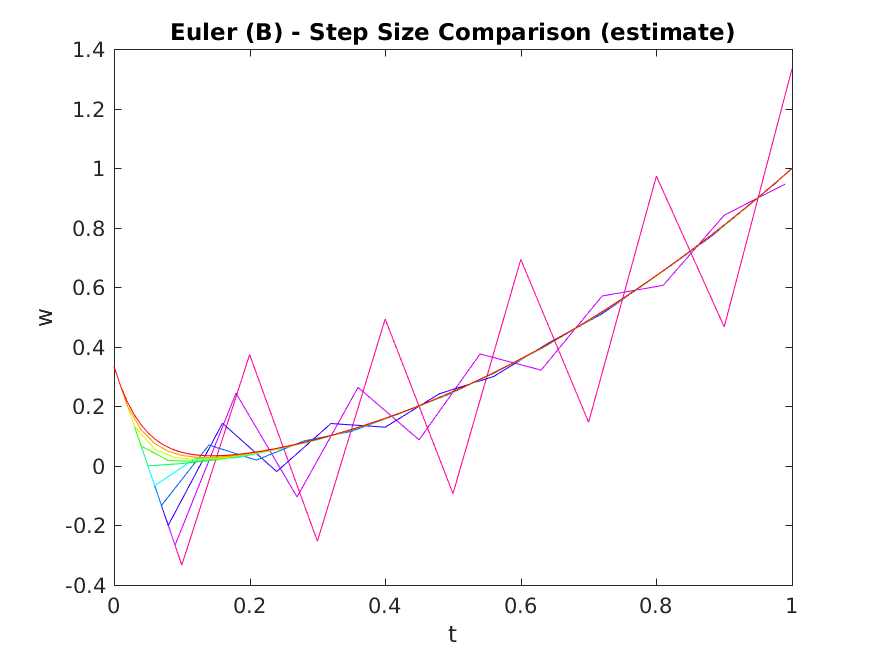
\includegraphics[width=1\textwidth]{../output/b_euler_h_val.png}
    \end{minipage}
   	\captionof{figure}{IVP A and B solution estimates for range of step sizes}
 	\label{fig:euler_h_val}
\end{center}

For both IVPs A and B remain stable when using a step size of 0.1 or smaller. IVP B does border on instability with a step size of 0.1, as can be seen in Figure \ref{fig:euler_h_val}, but improve significantly as the step size decreases. IVP A does suffer slightly with step sizes near 0.1, though not as drastically as IVP B. As would be expected, the borderline instability of IVP B with a step size of 0.1 results in larger error values, shown in Figure \ref{fig:euler_h_err}.

\begin{center}
	\centering
    \begin{minipage}{0.5\textwidth}
        \centering
	    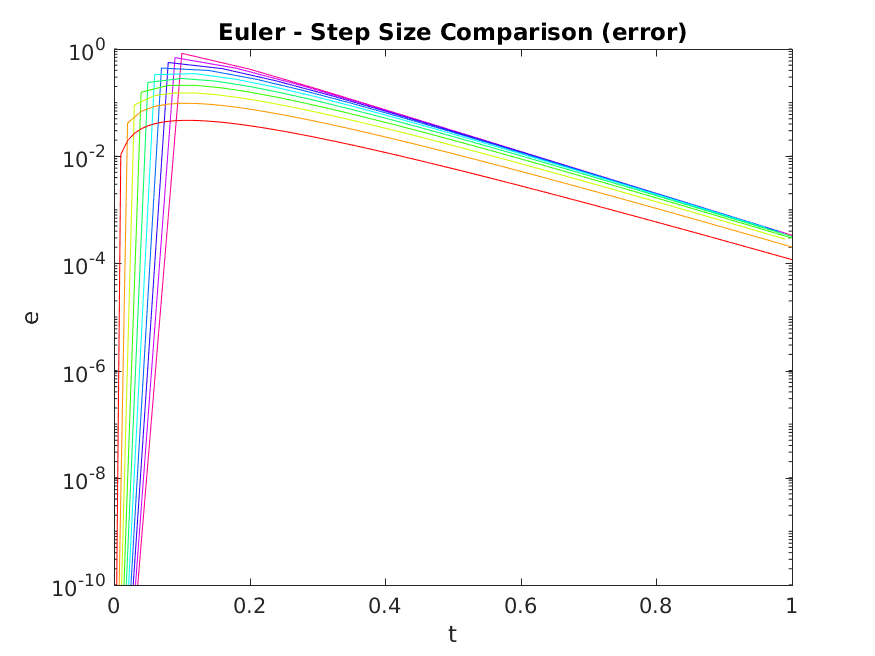
\includegraphics[width=1\textwidth]{../output/a_euler_h_err.png}
    \end{minipage}\hfill
    \begin{minipage}{0.5\textwidth}
        \centering
	    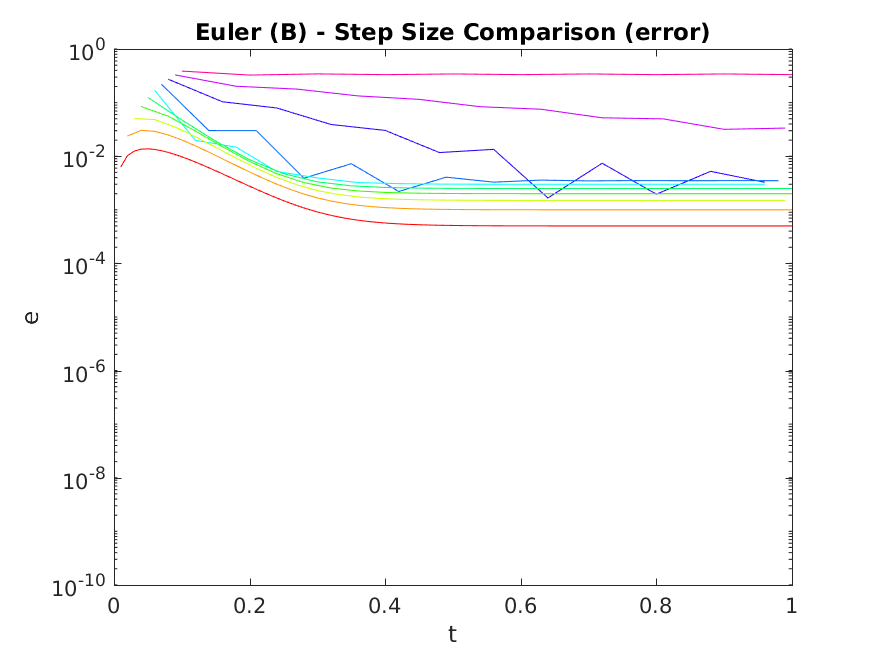
\includegraphics[width=1\textwidth]{../output/b_euler_h_err.png}
    \end{minipage}
   	\captionof{figure}{IVP A and B solution estimate error for range of step sizes}
 	\label{fig:euler_h_err}
\end{center}

In Tables \ref{tab:a_euler} and \ref{tab:b_euler} the resulting estimate and error values for a step size of 0.1 are listed. The consistent or slightly decreasing error values are indicative of stability at this step size.

\begin{table}[H]
\footnotesize
\centering
\caption{Euler's Results for A (h=0.1)}
\label{tab:a_euler}
\begin{tabular}{rrrrl}
\textbf{t} & \textbf{true} & \textbf{estimate} & \textbf{error} &  \\
0          & 2.7182818     & 2.7182818      & 4.4408921E-016  &  \\
0.1        & 1.1051709     & 0.27182818     & 0.83334274      &  \\
0.2        & 0.44932896    & 0.027182818    & 0.42214615      &  \\
0.3        & 0.18268352    & 0.0027182818   & 0.17996524      &  \\
0.4        & 0.074273578   & 0.0002718282   & 0.07400175      &  \\
0.5        & 0.030197383   & 2.7182818E-005 & 0.030170201     &  \\
0.6        & 0.01227734    & 2.7182818E-006 & 0.012274622     &  \\
0.7        & 0.0049915939  & 2.7182818E-007 & 0.0049913221    &  \\
0.8        & 0.0020294306  & 2.7182818E-008 & 0.0020294035    &  \\
0.9        & 0.0008251049  & 2.7182818E-009 & 0.0008251022    &  \\
1          & 0.0003354626  & 2.7182818E-010 & 0.0003354624    
\end{tabular}
\end{table}

\begin{table}[H]
\footnotesize
\centering
\caption{Euler's Results for B (h=0.1)}
\label{tab:b_euler}
\begin{tabular}{rrrrl}
\textbf{t} & \textbf{true} & \textbf{estimate} & \textbf{error} &  \\
0          & 0.33333333    & 0.33333333     & 0               &  \\
0.1        & 0.055111761   & -0.33333333    & 0.38844509      &  \\
0.2        & 0.046105213   & 0.37333333     & 0.32722812      &  \\
0.3        & 0.090826251   & -0.25333333    & 0.34415958      &  \\
0.4        & 0.16011182    & 0.49333333     & 0.33322151      &  \\
0.5        & 0.25001513    & -0.093333333   & 0.34334847      &  \\
0.6        & 0.36000205    & 0.69333333     & 0.33333129      &  \\
0.7        & 0.49000028    & 0.14666667     & 0.34333361      &  \\
0.8        & 0.64000004    & 0.97333333     & 0.3333333       &  \\
0.9        & 0.81000001    & 0.46666667     & 0.34333334      &  \\
1          & 1             & 1.3333333      & 0.33333333      & 
\end{tabular}
\end{table}

When the step size is increased to 0.25 for A and 0.2 for B, Euler's method becomes unstable for these stiff equations. In both cases, the error continously increases, as seen in Tables \ref{tab:un_a_euler} and \ref{tab:un_b_euler}. Although the increase in error is not as drastic for IVP A, the estimated value is still orders of magnitude larger than the true value.

\begin{table}[H]
\footnotesize
\centering
\caption{Unstable Euler's Results for A}
\label{tab:un_a_euler}
\begin{tabular}{rrrr}
\textbf{t} & \textbf{true} & \textbf{value} & \textbf{error} \\
0          & 2.7182818     & 2.7182818      & 4.4408921E-016 \\
0.25       & 0.2865048     & -3.3978523     & 3.6843571      \\
0.5        & 0.030197383   & 4.2473154      & 4.217118       \\
0.75       & 0.0031827808  & -5.3091442     & 5.312327       \\
1          & 0.0003354626  & 6.6364302      & 6.6360948         
\end{tabular}
\end{table}

\begin{table}[H]
\footnotesize
\centering
\caption{Unstable Euler's Results for B}
\label{tab:un_b_euler}
\begin{tabular}{rrrr}
\textbf{t} & \textbf{true} & \textbf{value} & \textbf{error} \\
0          & 0.33333333    & 0.33333333     & 0              \\
0.2        & 0.046105213   & -1             & 1.0461052      \\
0.4        & 0.16011182    & 3.24           & 3.0798882      \\
0.6        & 0.36000205    & -8.92          & 9.280002       \\
0.8        & 0.64000004    & 28.44          & 27.8           \\
1          & 1             & -82.44         & 83.44         
\end{tabular}
\end{table}


%\begin{center}
%  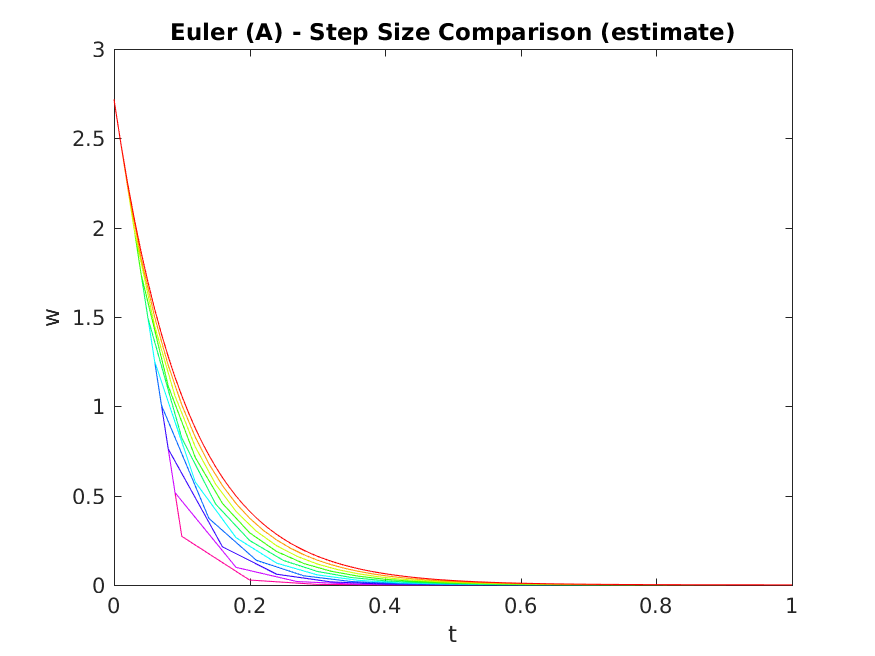
\includegraphics[width=0.9\textwidth]{../output/a_euler_h_val.png}
%  \captionof{figure}{a euler h val}
%  \label{fig:a_euler_h_val}
%\end{center}
%
%\begin{center}
%  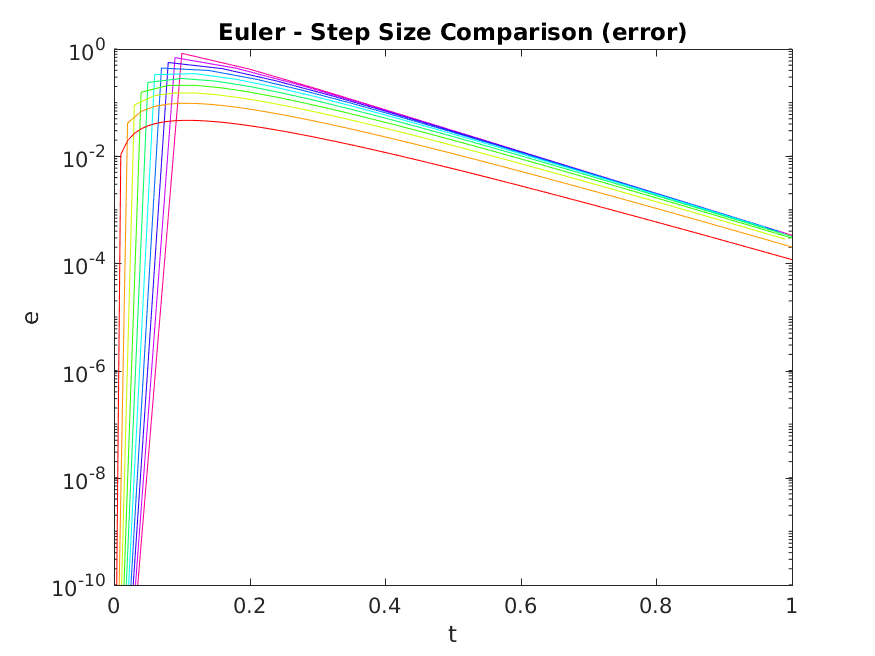
\includegraphics[width=0.9\textwidth]{../output/a_euler_h_err.png}
%  \captionof{figure}{a euler h err}
%  \label{fig:a_euler_h_err}
%\end{center}
%
%\begin{center}
%  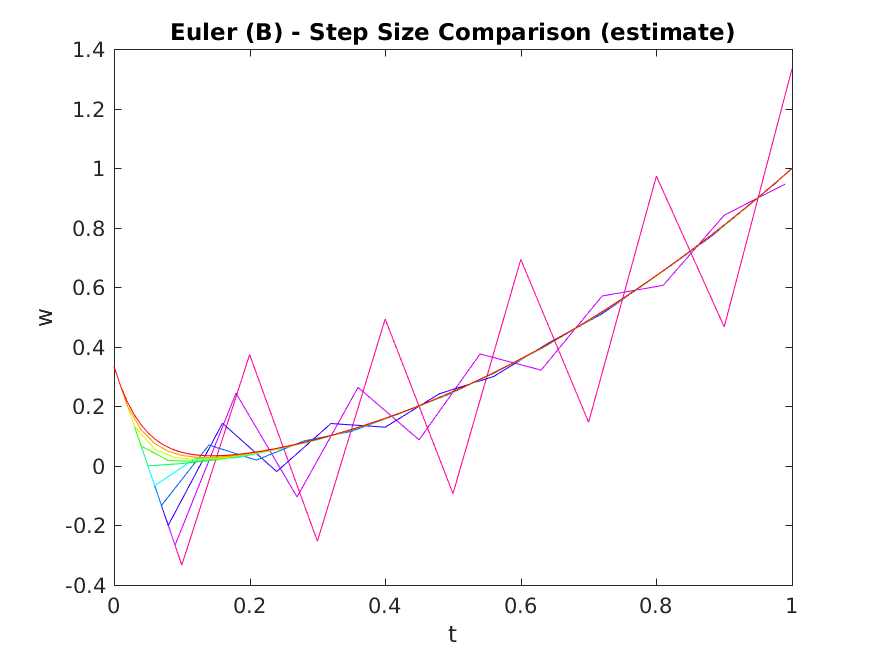
\includegraphics[width=0.9\textwidth]{../output/b_euler_h_val.png}
%  \captionof{figure}{b euler h val}
%  \label{fig:b_euler_h_val}
%\end{center}
%
%\begin{center}
%  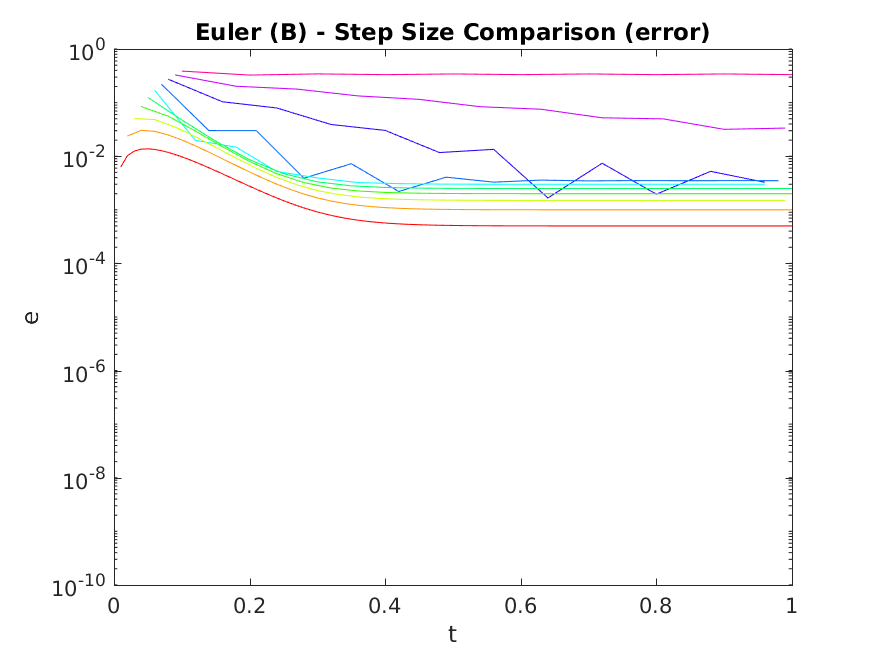
\includegraphics[width=0.9\textwidth]{../output/b_euler_h_err.png}
%  \captionof{figure}{b euler h err}
%  \label{fig:b_euler_h_err}
%\end{center}

\subsection{Runge-Kutta Results}
\label{results:rk}

\begin{center}
	\centering
    \begin{minipage}{0.5\textwidth}
        \centering
	    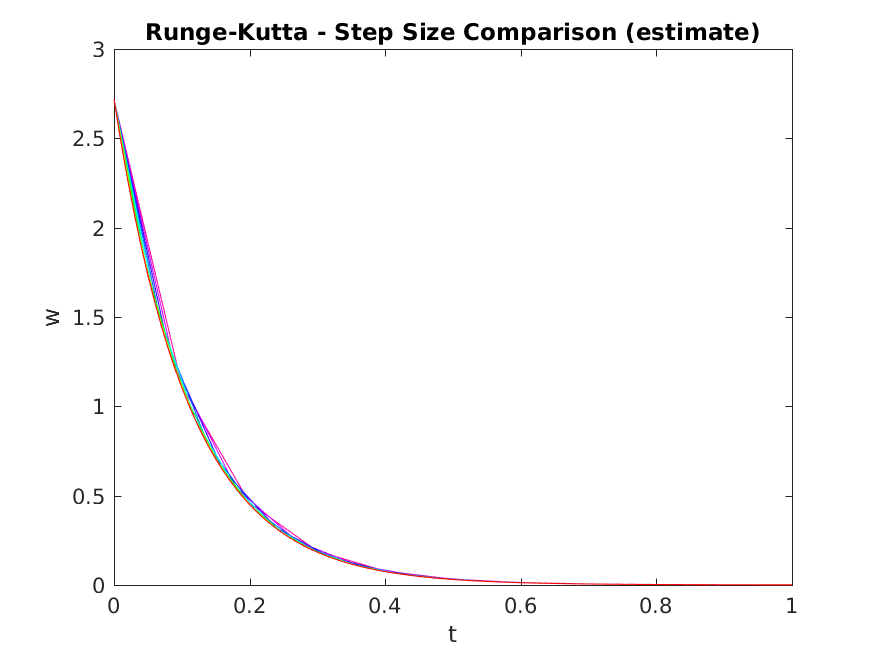
\includegraphics[width=1\textwidth]{../output/a_rk_h_val.png}
    \end{minipage}\hfill
    \begin{minipage}{0.5\textwidth}
        \centering
	    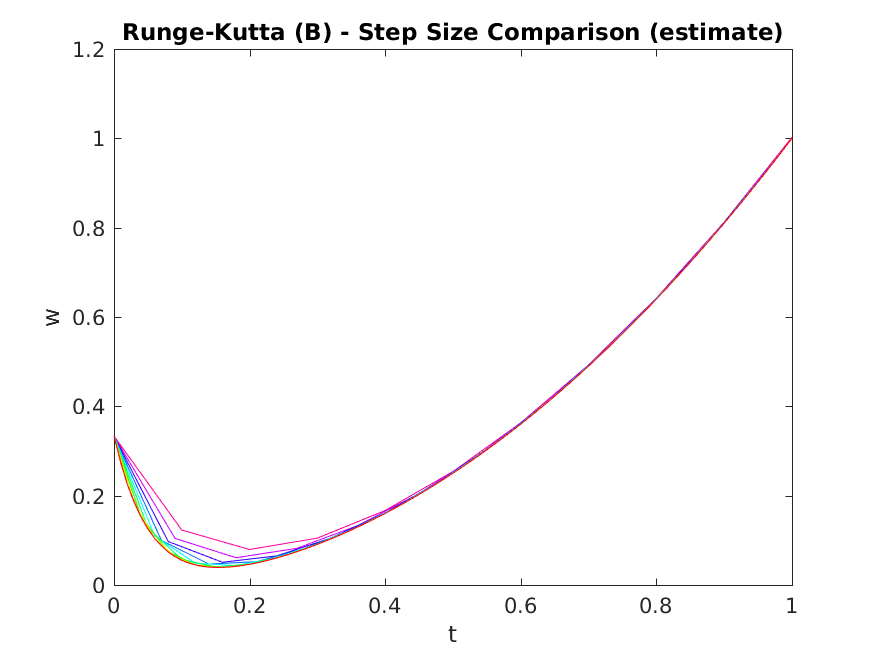
\includegraphics[width=1\textwidth]{../output/b_rk_h_val.png}
    \end{minipage}
   	\captionof{figure}{IVP A and B solution estimates for range of step sizes}
 	\label{fig:rk_h_val}
\end{center}

Over the range of step sizes betwen 0.01 and 0.1, the fourth order Runge-Kutta method is also stable. This method produced more accurate estimates than Euler's method, which is expected given than Euler's method is a low order Taylor's method, while the Runge-Kutta used is fourth order.

The solution estimates and corresponding error are plotted for the range of step sizes in Figures \ref{fig:rk_h_val} and \ref{fig:rk_h_err}, respectively
\begin{center}
	\centering
    \begin{minipage}{0.5\textwidth}
        \centering
	    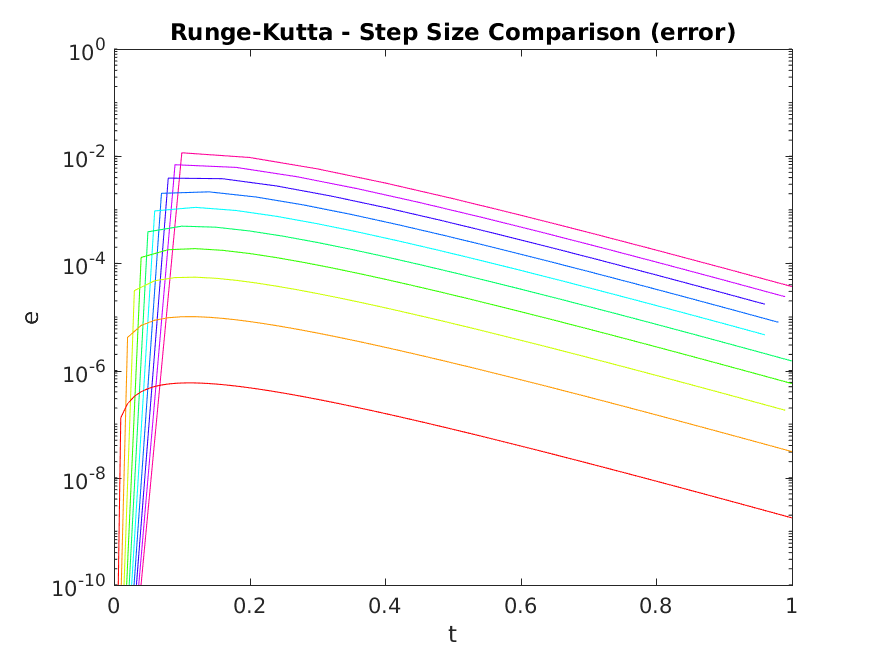
\includegraphics[width=1\textwidth]{../output/a_rk_h_err.png}
    \end{minipage}\hfill
    \begin{minipage}{0.5\textwidth}
        \centering
	    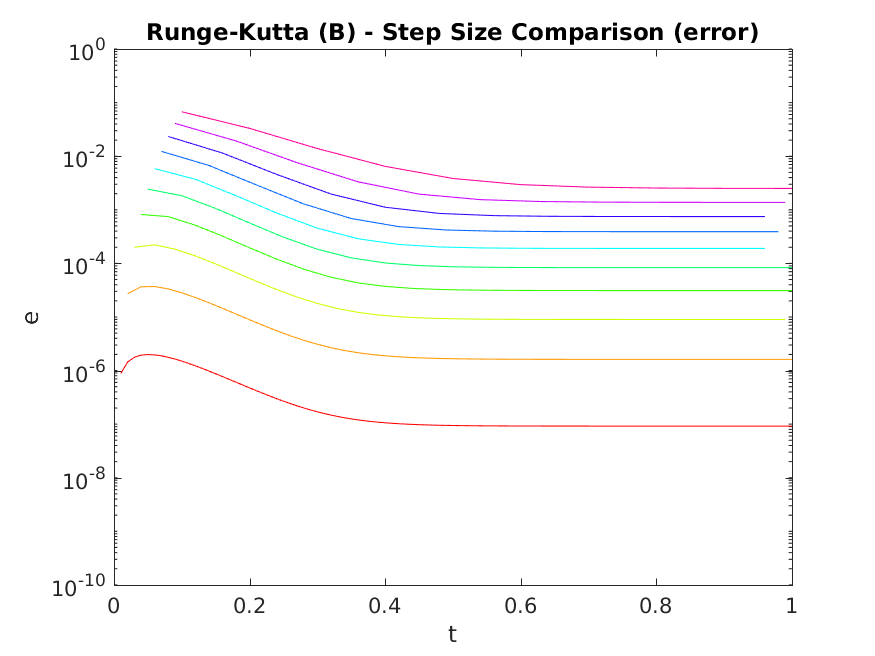
\includegraphics[width=1\textwidth]{../output/b_rk_h_err.png}
    \end{minipage}
   	\captionof{figure}{IVP A and B solution estimate error for range of step sizes}
 	\label{fig:rk_h_err}
\end{center}

As Figure \ref{fig:rk_h_err} shows, the error values listed in Tables \ref{tab:a_rk} and \ref{tab:b_rk} show consistent or slightly decreasing error, similar to Euler's method, indicating good stability at a step size of 0.1.

\begin{table}[H]
\footnotesize
\centering
\caption{Runge-Kutta Results for A}
\label{tab:a_rk}
\begin{tabular}{rrrrl}
\textbf{t} & \textbf{true} & \textbf{value} & \textbf{error} &  \\
0          & 2.7182818     & 2.7182818      & 4.4408921E-016 &  \\
0.1        & 1.1051709     & 1.1167721      & 0.011601193    &  \\
0.2        & 0.44932896    & 0.45881186     & 0.0094828979   &  \\
0.3        & 0.18268352    & 0.18849712     & 0.0058135943   &  \\
0.4        & 0.074273578   & 0.077441685    & 0.0031681067   &  \\
0.5        & 0.030197383   & 0.031815948    & 0.0016185648   &  \\
0.6        & 0.01227734    & 0.013071185    & 0.0007938447   &  \\
0.7        & 0.0049915939  & 0.0053701328   & 0.0003785389   &  \\
0.8        & 0.0020294306  & 0.0022062519   & 0.0001768213   &  \\
0.9        & 0.0008251049  & 0.000906411    & 0.000081306108 &  \\
1          & 0.0003354626  & 0.0003723876   & 0.000036925    
\end{tabular}
\end{table}


\begin{table}[H]
\footnotesize
\centering
\caption{Runge-Kutta Results for B}
\label{tab:b_rk}
\begin{tabular}{rrrrl}
\textbf{t} & \textbf{true} & \textbf{value} & \textbf{error} &  \\
0          & 0.33333333    & 0.33333333     & 0              &  \\
0.1        & 0.055111761   & 0.12277778     & 0.067666017    &  \\
0.2        & 0.046105213   & 0.079259259    & 0.033154046    &  \\
0.3        & 0.090826251   & 0.10475309     & 0.013926836    &  \\
0.4        & 0.16011182    & 0.16658436     & 0.0064725413   &  \\
0.5        & 0.25001513    & 0.25386145     & 0.0038463207   &  \\
0.6        & 0.36000205    & 0.36295382     & 0.0029517699   &  \\
0.7        & 0.49000028    & 0.49265127     & 0.0026509955   &  \\
0.8        & 0.64000004    & 0.64255042     & 0.0025503867   &  \\
0.9        & 0.81000001    & 0.81251681     & 0.002516803    &  \\
1          & 1             & 1.0025056      & 0.002505602    & 
\end{tabular}
\end{table}


When step size is increased to 0.25 for A and 0.2 for B, the Runge-Kutta method also becomes unstable for these stiff equations. IVP A, again, has less pronounced instability, though estimates are still order of magnitude greater than the true solution.


\begin{table}[H]
\footnotesize
\centering
\caption{Unstable Runge-Kutta Results for A}
\label{tab:un_a_rk}
\begin{tabular}{rrrr}
\textbf{t} & \textbf{true} & \textbf{value} & \textbf{error} \\
0          & 2.7182818     & 2.7182818      & 4.4408921E-016 \\
0.25       & 0.2865048     & 1.225085       & 0.93858023     \\
0.5        & 0.030197383   & 0.55212572     & 0.52192834     \\
0.75       & 0.0031827808  & 0.248834       & 0.24565122     \\
1          & 0.0003354626  & 0.1121454      & 0.11180994        
\end{tabular}
\end{table}

\begin{table}[H]
\footnotesize
\centering
\caption{Unstable Runge-Kutta Results for B}
\label{tab:un_b_rk}
\begin{tabular}{rrrr}
\textbf{t} & \textbf{true} & \textbf{value} & \textbf{error} \\
0          & 0.33333333    & 0.33333333     & 0              \\
0.2        & 0.046105213   & 1.76           & 1.7138948      \\
0.4        & 0.16011182    & 8.8133333      & 8.6532215      \\
0.6        & 0.36000205    & 43.68          & 43.319998      \\
0.8        & 0.64000004    & 217.29333      & 216.65333      \\
1          & 1             & 1084.32        & 1083.32       
\end{tabular}
\end{table}


%\begin{center}
%  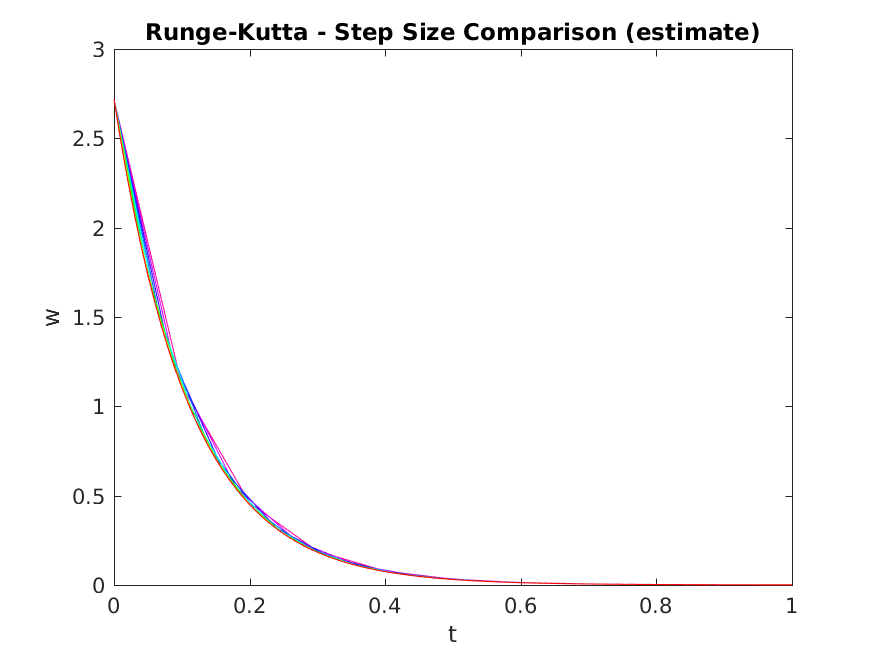
\includegraphics[width=0.9\textwidth]{../output/a_rk_h_val.png}
%  \captionof{figure}{a rk h val}
%  \label{fig:a_rk_h_val}
%\end{center}
%
%\begin{center}
%  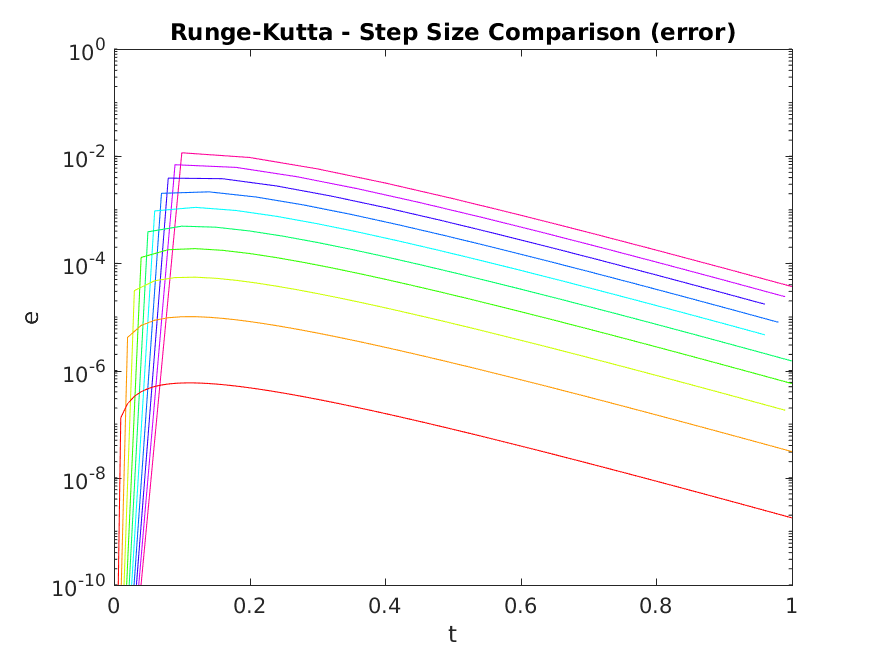
\includegraphics[width=0.9\textwidth]{../output/a_rk_h_err.png}
%  \captionof{figure}{a rk h err}
%  \label{fig:a_rk_h_err}
%\end{center}
%
%\begin{center}
%  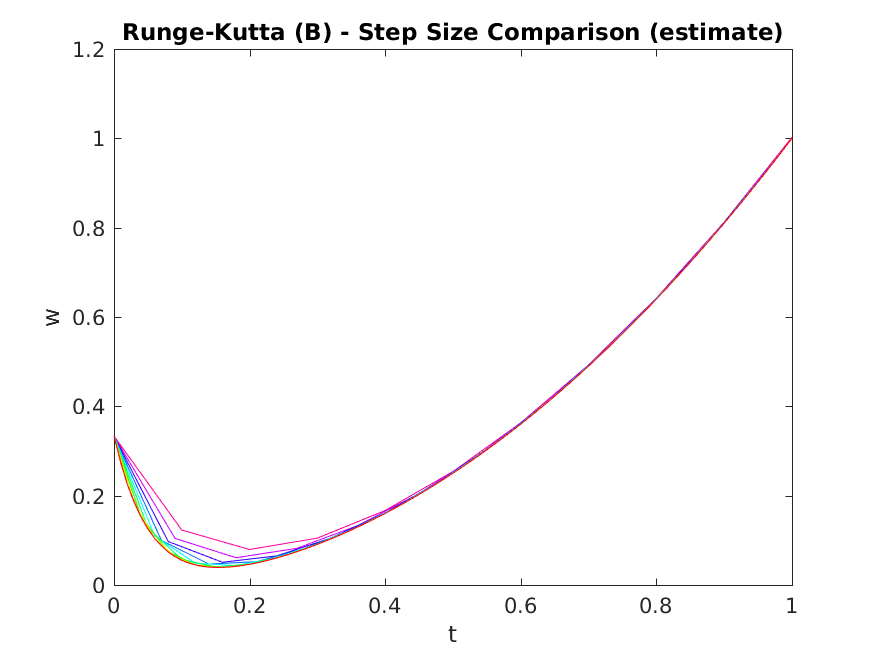
\includegraphics[width=0.9\textwidth]{../output/b_rk_h_val.png}
%  \captionof{figure}{b rk h val}
%  \label{fig:b_rk_h_val}
%\end{center}
%
%\begin{center}
%  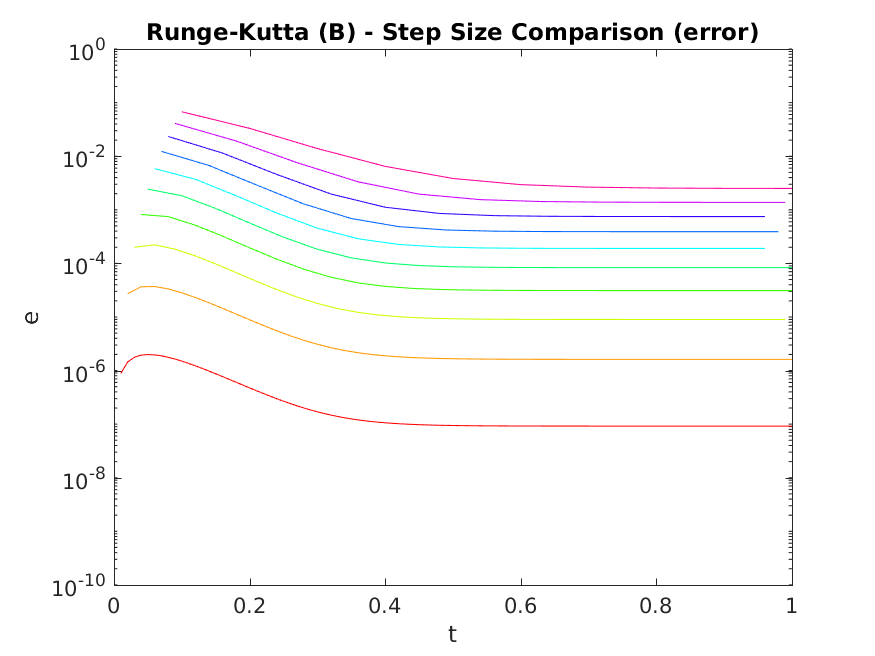
\includegraphics[width=0.9\textwidth]{../output/b_rk_h_err.png}
%  \captionof{figure}{b rk h err}
%  \label{fig:b_rk_h_err}
%\end{center}

\subsection{Implicit Trapezoidal Results}
\label{results:implicit}

\begin{center}
	\centering
    \begin{minipage}{0.5\textwidth}
        \centering
	    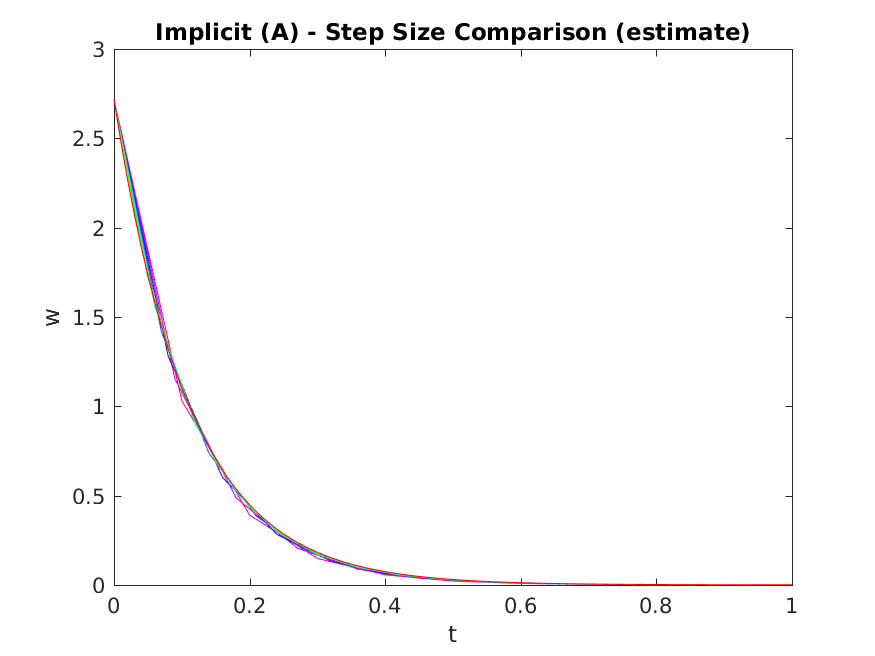
\includegraphics[width=1\textwidth]{../output/a_implicit_h_val.png}
    \end{minipage}\hfill
    \begin{minipage}{0.5\textwidth}
        \centering
	    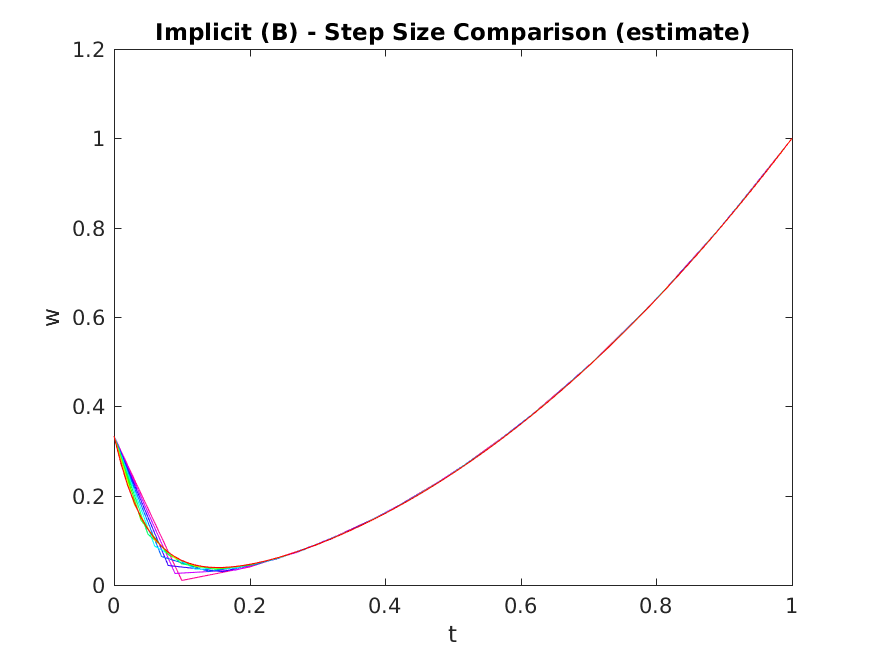
\includegraphics[width=1\textwidth]{../output/b_implicit_h_val.png}
    \end{minipage}
   	\captionof{figure}{IVP A and B solution estimates for range of step sizes}
 	\label{fig:implicit_h_val}
\end{center}

Using steps sizes between 0.01 and 0.1 the implicit method exibits similar stability and accuracy compared to the Runge-Kutta fourth order method. The plots for solution estimates and error can be seen in Figures \ref{fig:implicit_h_val} and \ref{fig:implicit_h_err}.

\begin{center}
	\centering
    \begin{minipage}{0.5\textwidth}
        \centering
	    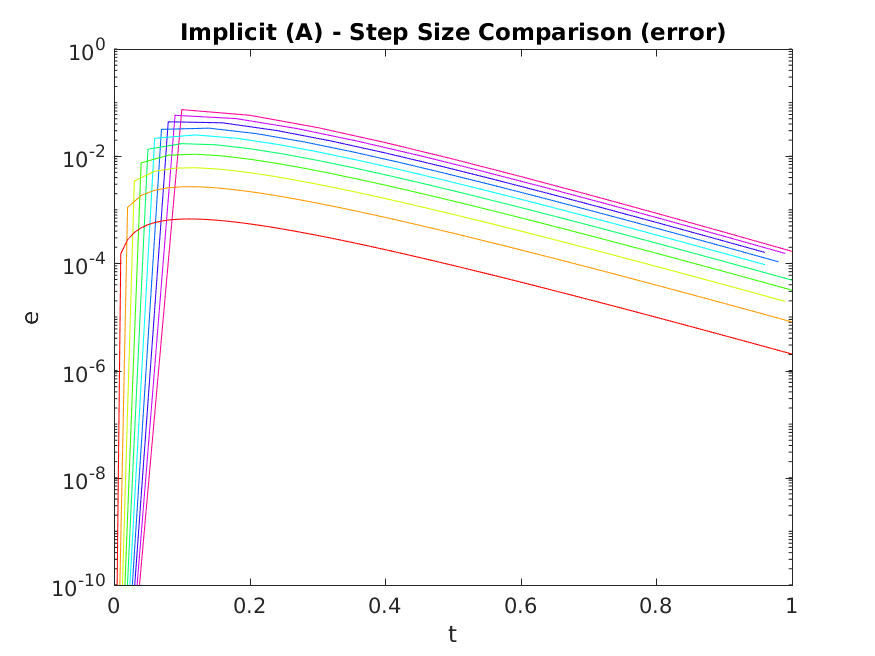
\includegraphics[width=1\textwidth]{../output/a_implicit_h_err.png}
    \end{minipage}\hfill
    \begin{minipage}{0.5\textwidth}
        \centering
	    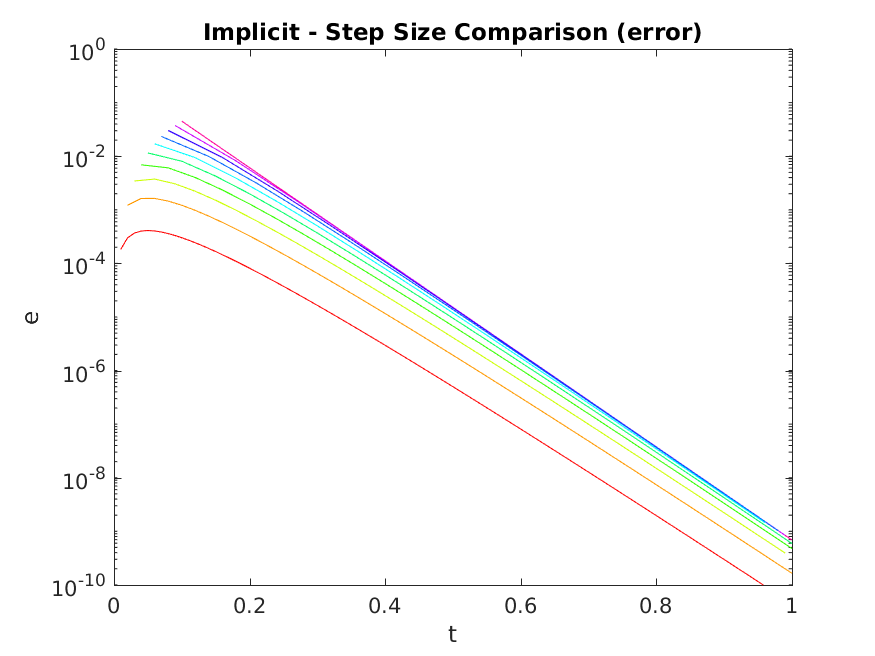
\includegraphics[width=1\textwidth]{../output/b_implicit_h_err.png}
    \end{minipage}
   	\captionof{figure}{IVP A and B solution estimate error for range of step sizes}
 	\label{fig:implicit_h_err}
\end{center}

Tables \ref{tab:a_implcit} and \ref{tab:b_implcit} detail the estimates and error for step size of 0.1.

\begin{table}[H]
\footnotesize
\centering
\caption{Implicit Trapezoidal Results for A}
\label{tab:a_implcit}
\begin{tabular}{rrrrl}
\textbf{t} & \textbf{true} & \textbf{value} & \textbf{error} &  \\
0          & 2.7182818     & 2.7182818      & 4.4408921E-016 &  \\
0.1        & 1.1051709     & 1.0310724      & 0.0740985      &  \\
0.2        & 0.44932896    & 0.39109643     & 0.05823253     &  \\
0.3        & 0.18268352    & 0.14834692     & 0.034336601    &  \\
0.4        & 0.074273578   & 0.056269523    & 0.018004056    &  \\
0.5        & 0.030197383   & 0.021343612    & 0.0088537714   &  \\
0.6        & 0.01227734    & 0.0080958528   & 0.0041814871   &  \\
0.7        & 0.0049915939  & 0.0030708407   & 0.0019207532   &  \\
0.8        & 0.0020294306  & 0.0011648017   & 0.000864629    &  \\
0.9        & 0.0008251049  & 0.0004418213   & 0.0003832836   &  \\
1          & 0.0003354626  & 0.0001675874   & 0.0001678752   
\end{tabular}
\end{table}


\begin{table}[H]
\footnotesize
\centering
\caption{Implicit Trapezoidal Results for B}
\label{tab:b_implcit}
\begin{tabular}{rrrrl}
\textbf{t} & \textbf{true} & \textbf{value} & \textbf{error} &  \\
0          & 0.33333333    & 0.33333333     & 0              &  \\
0.1        & 0.055111761   & 0.01           & 0.045111761    &  \\
0.2        & 0.046105213   & 0.04           & 0.006105213    &  \\
0.3        & 0.090826251   & 0.09           & 0.0008262507   &  \\
0.4        & 0.16011182    & 0.16           & 0.0001118209   &  \\
0.5        & 0.25001513    & 0.25           & 1.513331E-005  &  \\
0.6        & 0.36000205    & 0.36           & 2.0480708E-006 &  \\
0.7        & 0.49000028    & 0.49           & 2.7717624E-007 &  \\
0.8        & 0.64000004    & 0.64           & 3.7511725E-008 &  \\
0.9        & 0.81000001    & 0.81           & 5.0766599E-009 &  \\
1          & 1             & 1              & 6.870513E-010  & 
\end{tabular}
\end{table}

Even when the step size is increased to same size that caused instability when using Euler's and Runge-Kutta methods, the implicit method remained stable. It is worth noting that the accuracy when using a large step size is slightly reduced. The accuracy of the implcit trapezoidal method with Newtonian iteration and the associated error under stable conditions despite a larger step size can be seen in Tables \ref{tab:un_a_implicit} and \ref{tab:un_b_implicit},

\begin{table}[H]
\footnotesize
\centering
\caption{Stable Implicit Results for A}
\label{tab:un_a_implicit}
\begin{tabular}{rrrr}
\textbf{t} & \textbf{true} & \textbf{value} & \textbf{error} \\
0          & 2.7182818     & 2.7182818      & 4.4408921E-016 \\
0.25       & 0.2865048     & -0.15989893    & 0.44640373     \\
0.5        & 0.030197383   & 0.0094058195   & 0.020791564    \\
0.75       & 0.0031827808  & -0.0005532835  & 0.0037360643   \\
1          & 0.0003354626  & 0.000032546088 & 0.0003029165   
\end{tabular}
\end{table}

\begin{table}[H]
\footnotesize
\centering
\caption{Stable Implicit Results for B}
\label{tab:un_b_implicit}
\begin{tabular}{rrrr}
\textbf{t} & \textbf{true} & \textbf{value} & \textbf{error} \\
0          & 0.33333333    & 0.33333333     & 0              \\
0.2        & 0.046105213   & -0.071111111   & 0.11721632     \\
0.4        & 0.16011182    & 0.19703704     & 0.036925216    \\
0.6        & 0.36000205    & 0.34765432     & 0.012347727    \\
0.8        & 0.64000004    & 0.64411523     & 0.0041151888   \\
1          & 1             & 0.99862826     & 0.0013717428  
\end{tabular}
\end{table}


%\begin{center}
%  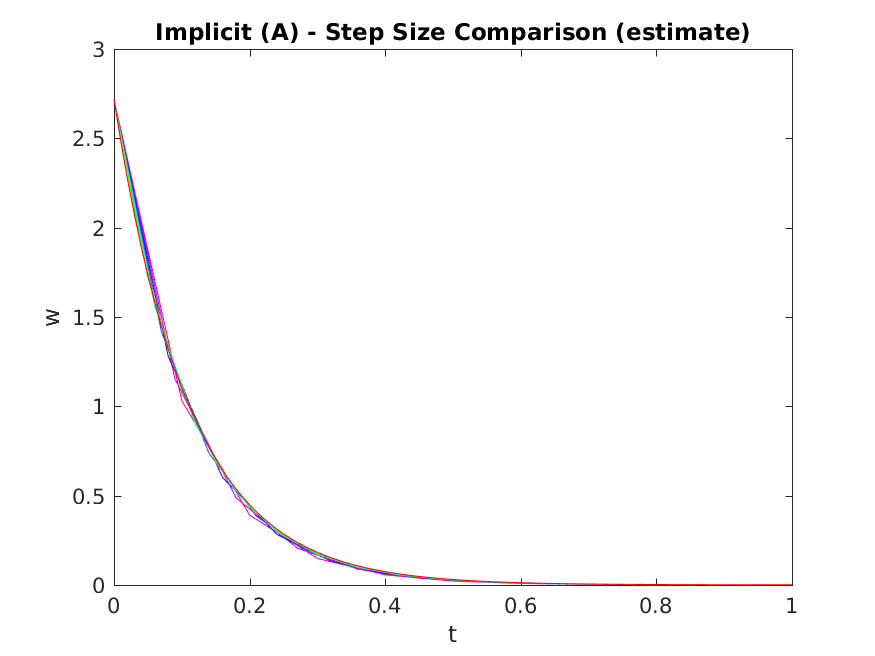
\includegraphics[width=0.9\textwidth]{../output/a_implicit_h_val.png}
%  \captionof{figure}{a implicit h val}
%  \label{fig:a_implicit_h_val}
%\end{center}
%
%\begin{center}
%  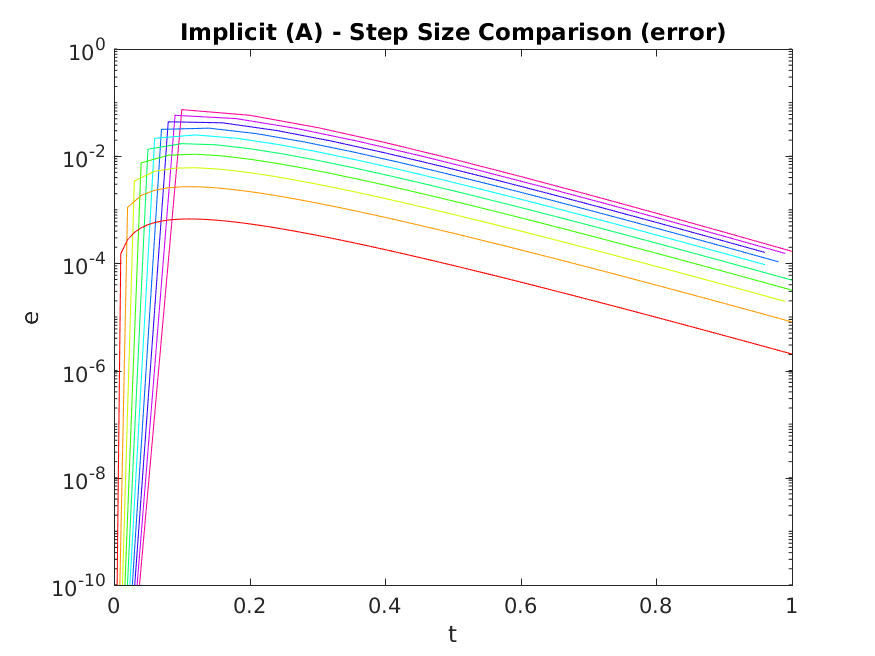
\includegraphics[width=0.9\textwidth]{../output/a_implicit_h_err.png}
%  \captionof{figure}{a implicit h err}
%  \label{fig:a_implicit_h_err}
%\end{center}
%
%\begin{center}
%  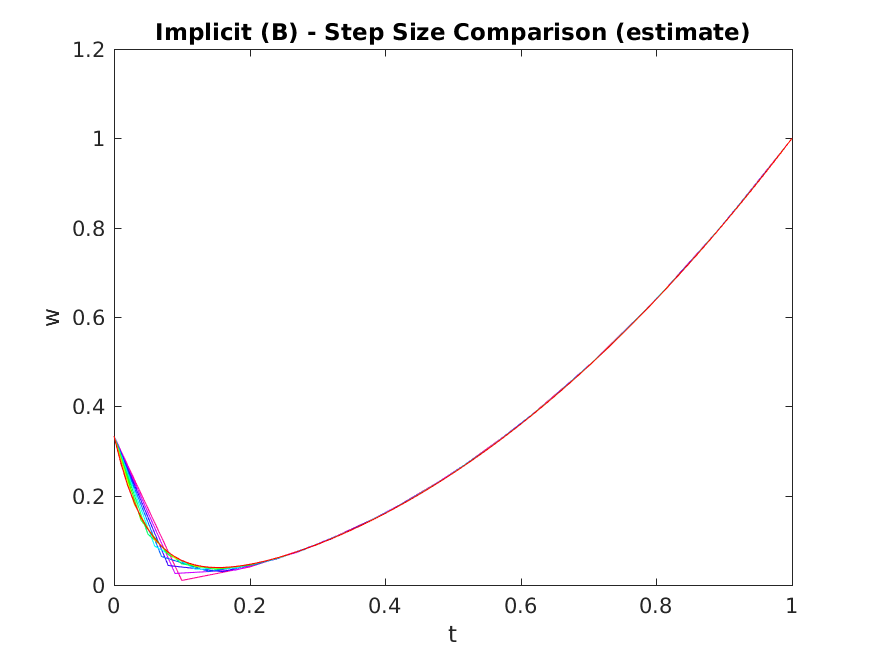
\includegraphics[width=0.9\textwidth]{../output/b_implicit_h_val.png}
%  \captionof{figure}{b implicit h val}
%  \label{fig:b_implicit_h_val}
%\end{center}
%
%\begin{center}
%  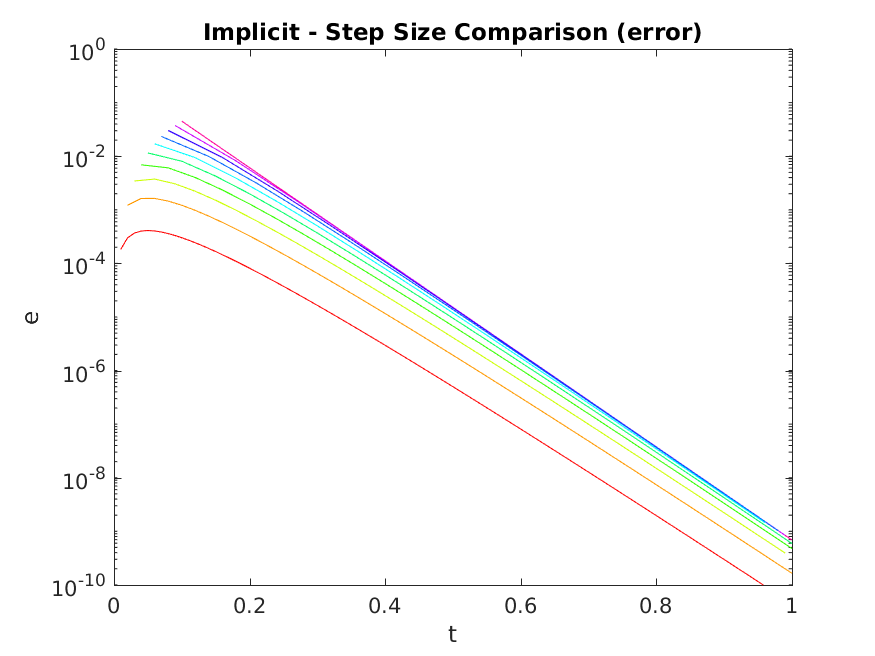
\includegraphics[width=0.9\textwidth]{../output/b_implicit_h_err.png}
%  \captionof{figure}{b implicit h err}
%  \label{fig:b_implicit_h_err}
%\end{center}


\section{Discussion and Conclusions}
\label{sec:conc}

This project explored different numerical methods of solving well-posed initial value problems (IVPs) at discrete points within a range for a given initial value. Section \ref{sec:methods} introduced the set of IVPs to be tested and the numerical methods for solving them. Section \ref{sec:results} presented the results from implementing each method using a range of step sizes to solve the IVPs.


\begin{center}
	\centering
    \begin{minipage}{0.5\textwidth}
        \centering
	    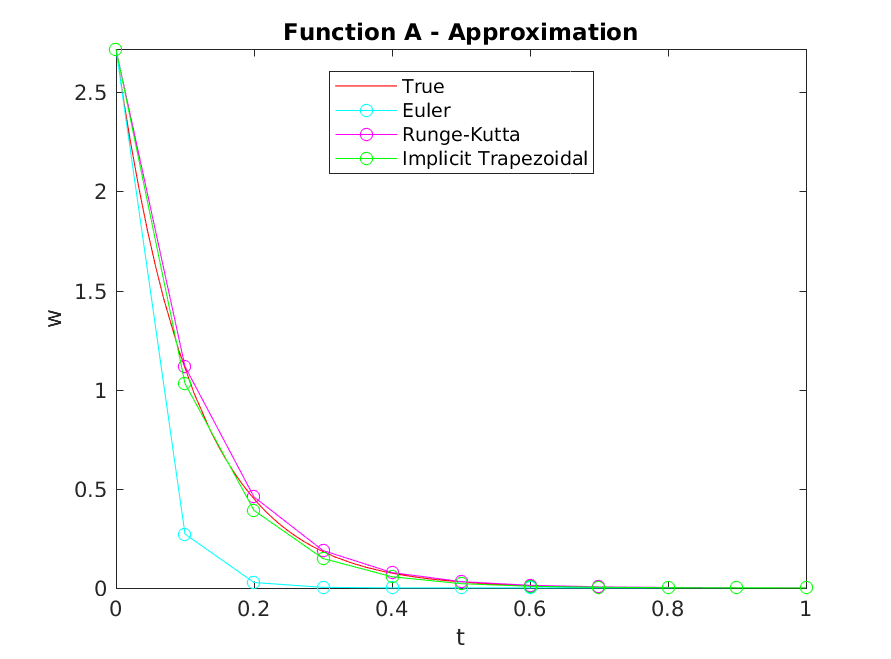
\includegraphics[width=1\textwidth]{../output/a_compare_val.png}
    \end{minipage}\hfill
    \begin{minipage}{0.5\textwidth}
        \centering
	    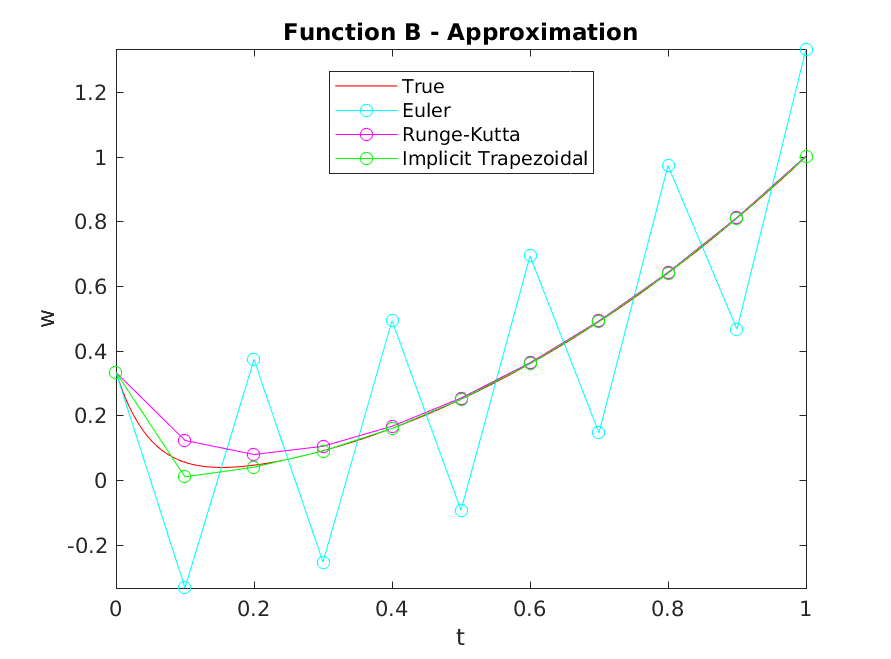
\includegraphics[width=1\textwidth]{../output/b_compare_val.png}
    \end{minipage}
   	\captionof{figure}{h=0.1}
 	\label{fig:compare_val}
\end{center}

Figure \ref{fig:compare_val} shows a comparison of each method with a step size of 0.1. For both IVP A and B, Euler's method is clearly the least accurate, followed by Runge-Kutta, with the implicit method providing the best results at this step size. The improved accuracy of the Runge-Kutta and the implcit methods are due to the fact that Euler's method is a low order implementation of Taylor's method. A higher order implementation of Taylor's method could be expected to provided more comparable levels of accuracy to the other methods. A detailed comparison is provided by \cite{burden2010}, showing that even with similar accuracy the fourth order Runge-Kutta method is more efficient than similar order Taylor's method. 

\begin{center}
	\centering
    \begin{minipage}{0.5\textwidth}
        \centering
	    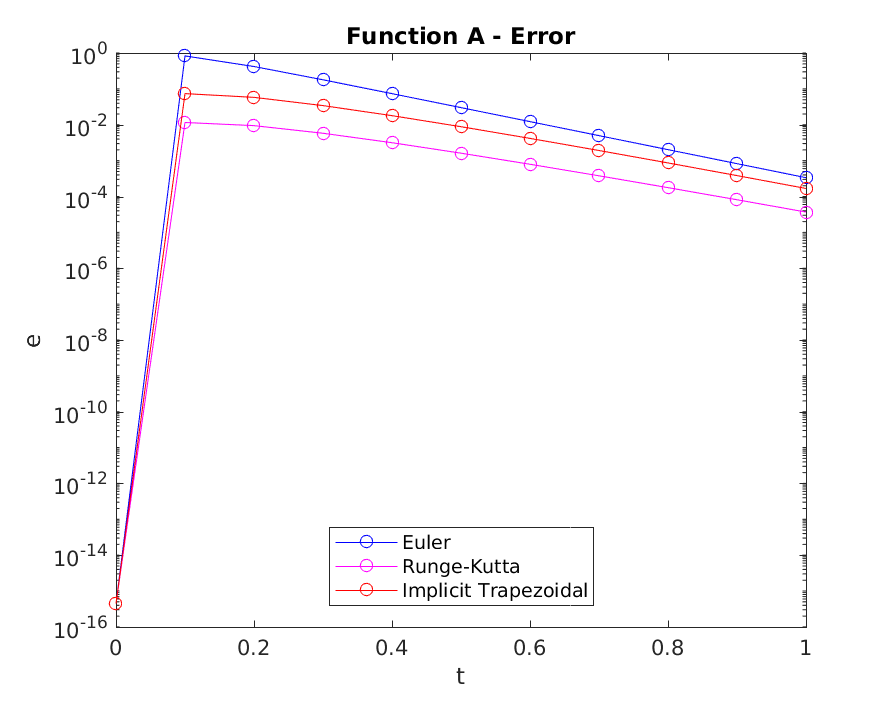
\includegraphics[width=1\textwidth]{../output/a_compare_err.png}
    \end{minipage}\hfill
    \begin{minipage}{0.5\textwidth}
        \centering
	    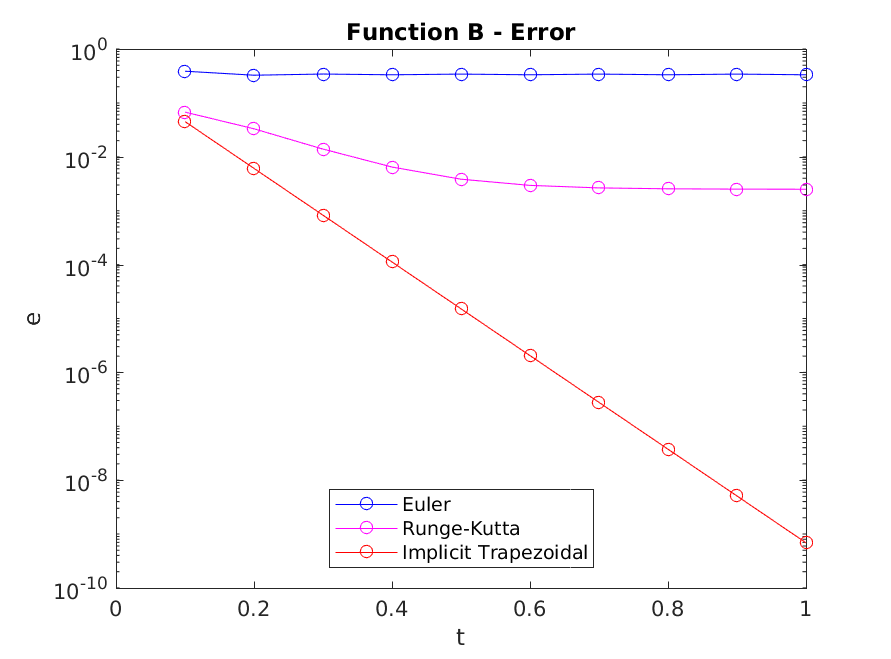
\includegraphics[width=1\textwidth]{../output/b_compare_err.png}
    \end{minipage}
   	\captionof{figure}{h=0.1}
 	\label{fig:compare_err}
\end{center}

Results from using varying step sizes in Section \ref{sec:results} illustrated the impact of step size when solving IVPs with stiff equations using explicit methods (Euler's and Runge-Kutta), and implcit methods (implicit trapezoidal with Newton Iteration). While using step size of 0.1 (Figure \ref{fig:compare_val}) or smaller, the explicit methods maintained stability. Increasing the step size to 0.25 and 0.2 for IVP A and B respectively caused both IVP solutions to become unstable, as seen in Figure \ref{fig:un_compare_val}.

xx

Implicit methods provide an alternative for solving IVPs with stiff equations that do not require reducing the step size.


discuss stability and step size for explicit methods
how stabiltiy can be improved by using smaller step sizes

What implicit means
How it impacts stability
How does it affect the solution to the IVPs and the step size

Discuss usage as solution to stability issues with Euler/RK

Even when the step size is increased using implicit method to same size that caused instability when using Euler's and Runge-Kutta methods, the implicit method remained stable. The accuracy is reduced for implicit method when using a large step size, but this is a minor trade-off for stability compared to the extremely large error and instability associated with one-step explicit methods when using large step sizes for stiff equations.


\begin{center}
	\centering
    \begin{minipage}{0.5\textwidth}
        \centering
	    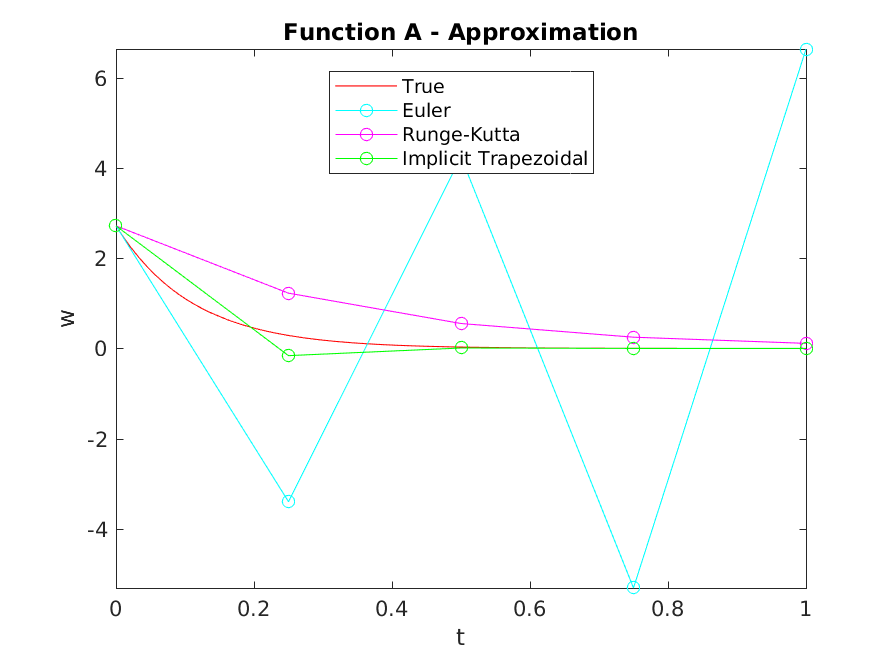
\includegraphics[width=1\textwidth]{../additional/unstable/a_compare_val.png}
    \end{minipage}\hfill
    \begin{minipage}{0.5\textwidth}
        \centering
	    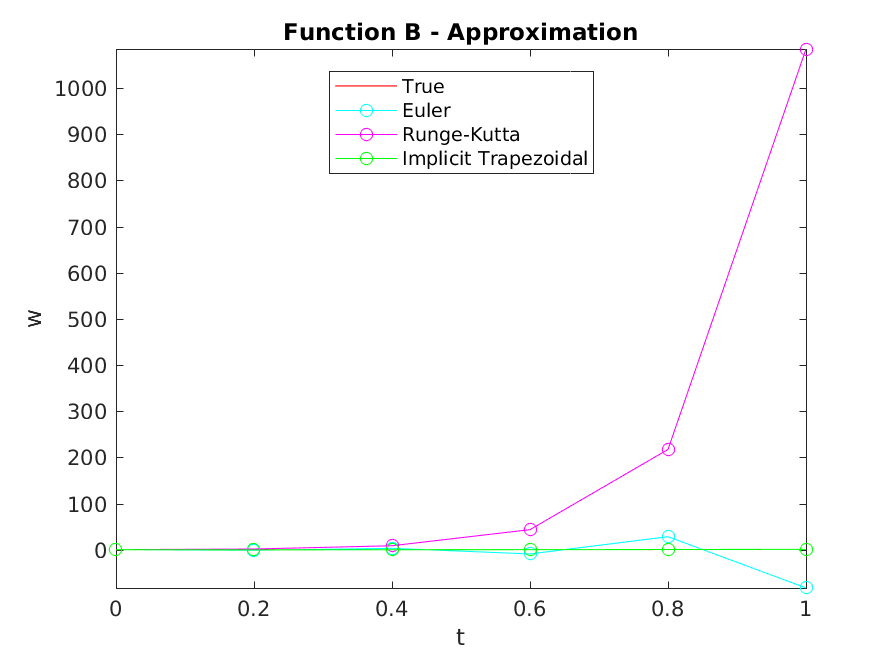
\includegraphics[width=1\textwidth]{../additional/unstable/b_compare_val.png}
    \end{minipage}
   	\captionof{figure}{h=0.25 (A) and 0.2 (B)}
 	\label{fig:un_compare_val}
\end{center}


%\begin{center}
%  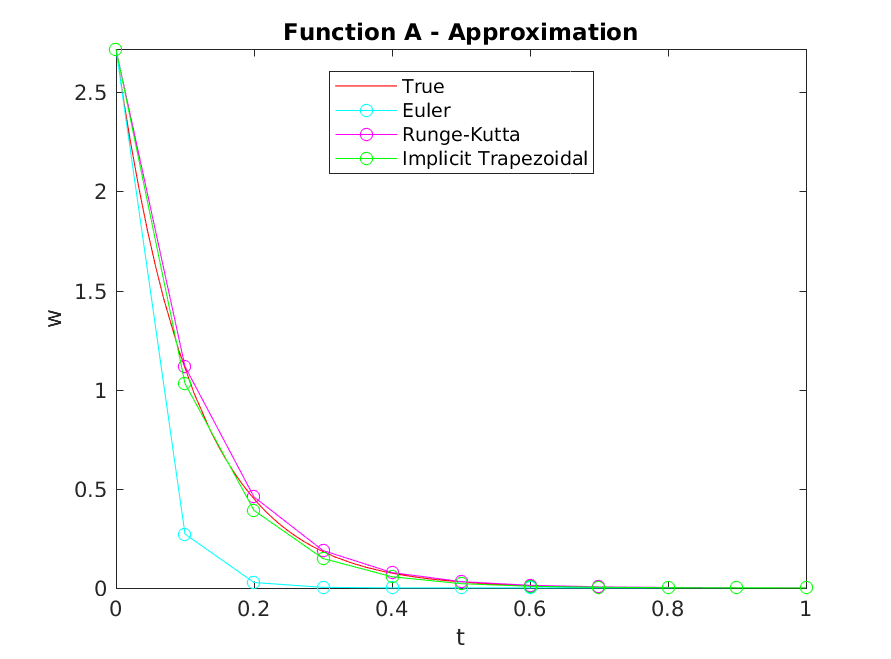
\includegraphics[width=0.9\textwidth]{../output/a_compare_val.png}
%  \captionof{figure}{a compare val}
%  \label{fig:a_compare_val}
%\end{center}
%
%\begin{center}
%  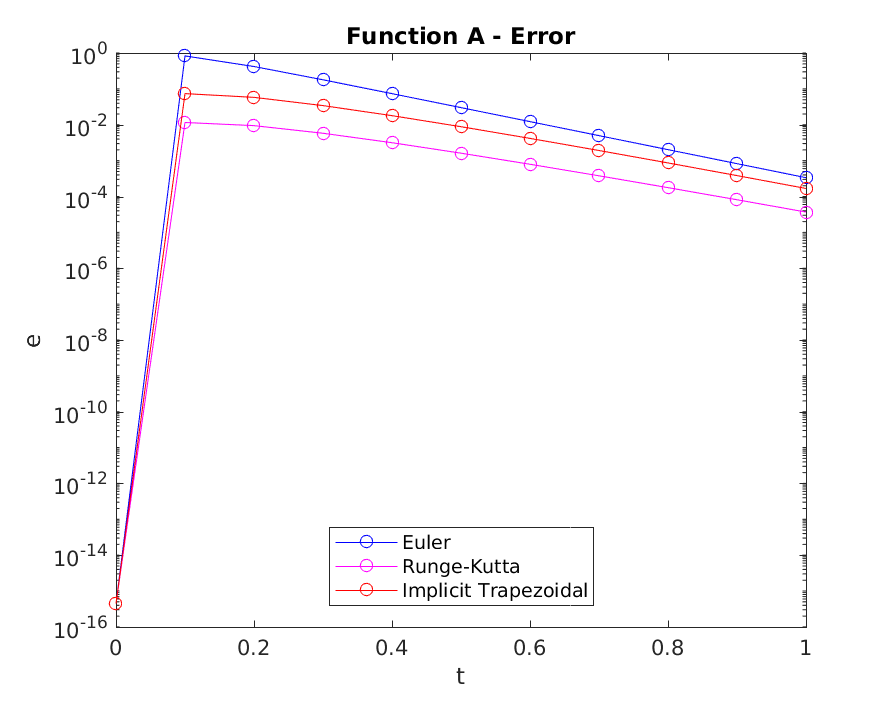
\includegraphics[width=0.9\textwidth]{../output/a_compare_err.png}
%  \captionof{figure}{a compare err}
%  \label{fig:a_compare_err}
%\end{center}
%
%\begin{center}
%  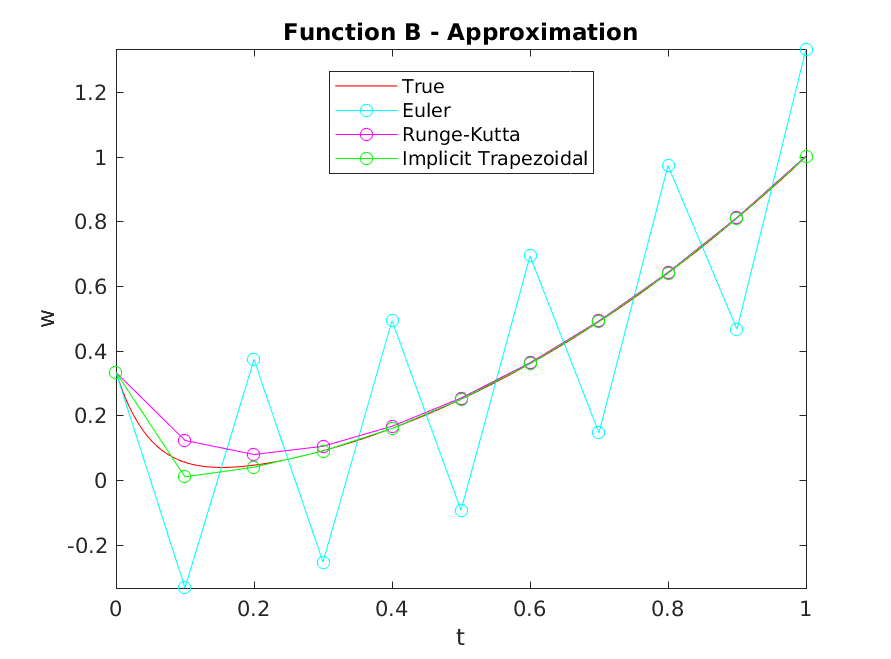
\includegraphics[width=0.9\textwidth]{../output/b_compare_val.png}
%  \captionof{figure}{b compare val}
%  \label{fig:b_compare_val}
%\end{center}
%
%\begin{center}
%  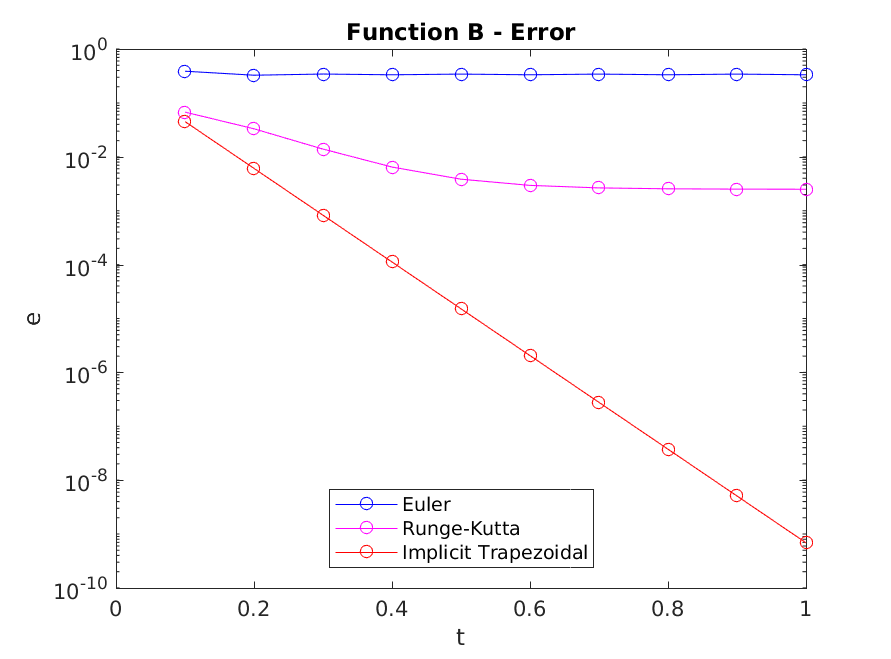
\includegraphics[width=0.9\textwidth]{../output/b_compare_err.png}
%  \captionof{figure}{b compare err}
%  \label{fig:b_compare_err}
%\end{center}

%\begin{center}
%  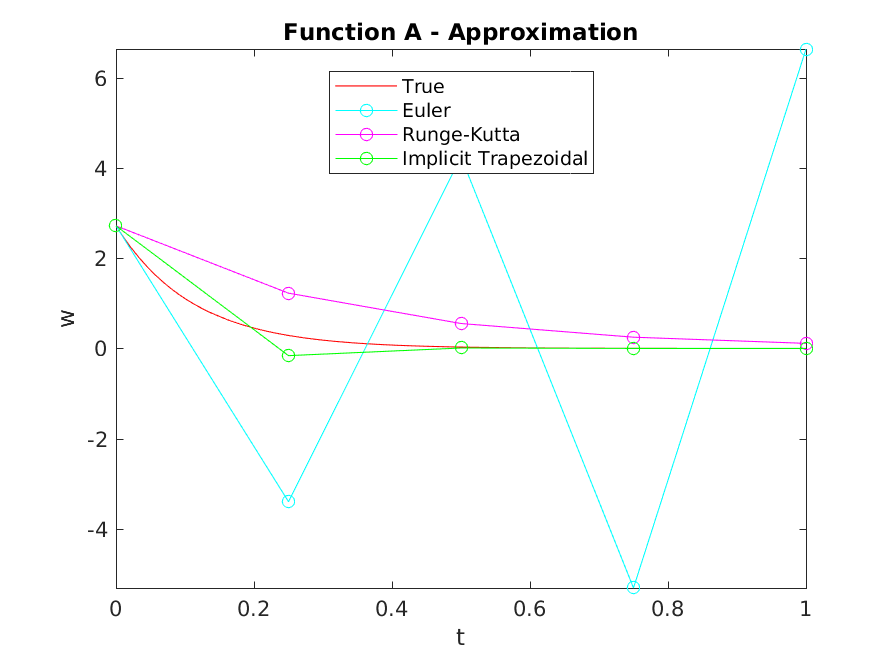
\includegraphics[width=0.9\textwidth]{../additional/unstable/a_compare_val.png}
%  \captionof{figure}{unstable a compare val}
%  \label{fig:un_a_compare_val}
%\end{center}
%
%\begin{center}
%  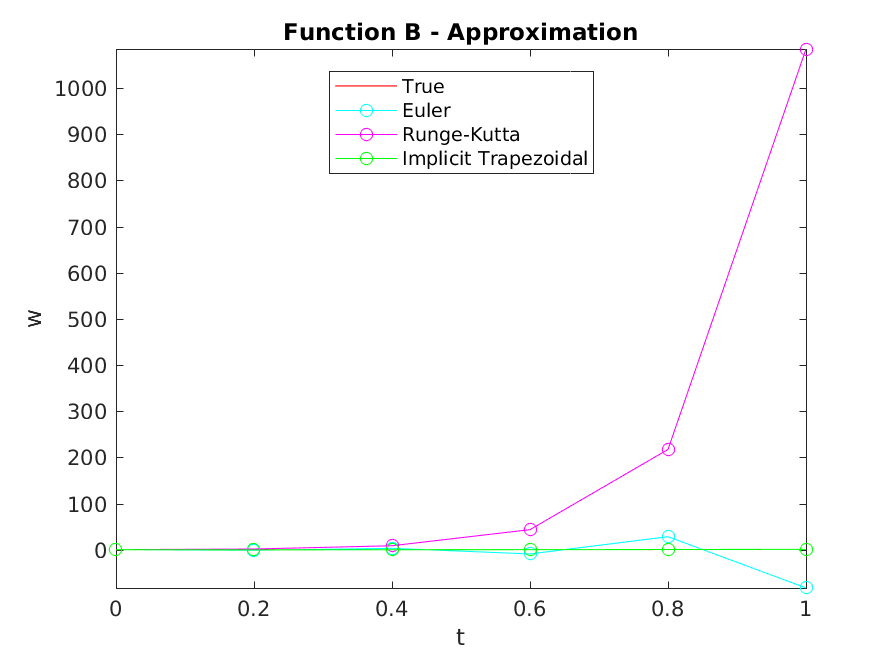
\includegraphics[width=0.9\textwidth]{../additional/unstable/b_compare_val.png}
%  \captionof{figure}{unstable a compare err}
%  \label{fig:un_a_compare_err}
%\end{center}


\newpage

\bibliography{report}


\end{document}
